\documentclass[a4paper,11pt]{article}

\usepackage{jinstpub} 
% for details on the use of the package, please
% see the JINST-author-manual
% https://jinst.sissa.it/jinst/help/JINST/TeXclass/jinst-author-manual.pdf

\usepackage[numbers,sort&compress]{natbib}
%\bibliographystyle{abbrvnat}
\bibliographystyle{unsrtnat}

\usepackage{physics}
\usepackage{siunitx}
\usepackage{lineno}
\usepackage{graphicx, subfigure}
\linenumbers

\usepackage{soul}
\usepackage{color}
\newcommand{\hlcyan}[1]{{\sethlcolor{cyan}\hl{#1}}}
\newcommand{\hlgreen}[1]{{\sethlcolor{green}\hl{#1}}}
\newcommand{\hlred}[1]{{\sethlcolor{red}\hl{#1}}}
\newcommand{\hlblue}[1]{{\sethlcolor{blue}\hl{#1}}}
\newcommand{\hlmag}[1]{{\sethlcolor{magenta}\hl{#1}}}

\title{\boldmath Front-end Electronics for the DUNE Photon Detection System.}


%% %simple case: 2 authors, same institution
%% \author{A. Uthor}
%% \author{and A. Nother Author}
%% \affiliation{Institution,\\Address, Country}

% more complex case: 4 authors, 3 institutions, 2 footnotes
\author[a,b,1]{F. Irst,\note{Corresponding author.}}
\author[c]{S. Econd,}
\author[a,2]{T. Hird\note{Also at Some University.}}
\author[c,2]{and Fourth}

% The "\note" macro will give a warning: "Ignoring empty anchor..."
% you can safely ignore it.

\affiliation[a]{One University,\\some-street, Country}
\affiliation[b]{Another University,\\different-address, Country}
\affiliation[c]{A School for Advanced Studies,\\some-location, Country}

% e-mail addresses: only for the corresponding author
\emailAdd{first@one.univ}




\abstract{Abstract...}



\keywords{Only keywords from JINST's keywords list please}


%\arxivnumber{1234.56789} % only if you have one


% \collaboration{\includegraphics[height=17mm]{example-image}\\[6pt]
%   XXX collaboration}
% or
\collaboration[c]{on behalf of the DUNE collaboration}
% The opiton "c" will give a warning, but only so that you can
% check that the output is what you expected

% if you write for a special issue this may be useful
%\proceeding{N$^{\text{th}}$ Workshop on X\\
%  when\\
%  where}



\begin{document}
\maketitle
\flushbottom

\section{Introduction}
\label{sec:introduction}

The Deep Underground Neutrino Experiment (DUNE) is an international experiment aimed to shed light on some of the mysteries at the forefront of particle physics and astrophysics via the precise measurement of neutrino oscillation parameters. The Far detector, located at SURF in South Dakota, consists of four gigantic modules with a total of \SI{40}{\kilo\tonne} of fiducial mass. Each module is a  liquid argon time-projection chamber (LArTPC) used for neutrino detection and signal reconstruction. \cite{Abi_2020,Abi_2020_2,Abi_2020_3}

In addition to the charge collection allowed by LArTPC technology, in DUNE is foreseen the implementation of a photon detection system (PDS), taking advantage of the scintillation properties of the Argon. For the two first DUNE Far detector Modules, the PDS technology is based on the ARAPUCA concept~\cite{Machado_2016}. The front-end system for the PDS first far detector is DAPHNE (Detector electronics for Acquiring PHotons from NEutrinos).

The current paper presents the system characteristics with a summary of the performance achieved in different labs. Finally,  we offer the plans for the PD readout implementation in ProtoDUNE-II.

%Table example
%\begin{table}[htbp]
%\centering
%\caption{\label{tab:i} We prefer that tables have the caption on top.}
%\smallskip
%\begin{tabular}{lrc}
%\hline
%x&y&x and y\\
%\hline
%a & b & a and b\\
%1 & 2 & 1 and 2\\
%$\alpha$ & $\beta$ & $\alpha$ and $\beta$\\
%\hline
%\end{tabular}
%\end{table}

\section{DAPHNE Front-End}
\label{sec:system}

DAPHNE is the front-end system for the Horizontal Drift Photon Detection System at DUNE. The signals from the XArapucas are amplified by a Cold Electronics system inside the TPC. These signals are transported by differential pairs to the warm side and digitized by DAPHNE. A trigger algorithm does the first discrimination of the signals in the FPGA. The Acquired data is sent to the DAQ system to Deploy in the LArSoft data frame.

\subsection{DAPHNE design}
\label{sec:requirements}

The design of the DAPHNE board is based on the Mu2e board (Cita) developed at Fermilab, from which it keeps the same architecture with an FPGA and a microcontroller, the core of the power supply, and the use of an analog front-end chip (AFE)~\cite{IEEE_Ref1:afe5808amanual}. Apart from the mentioned similarities, DAPHNE includes modifications concerning Mu2e, like the use of a different FPGA and microcontroller family, a total redesign of the voltage regulators block, and the upgraded model AFE5808A, among others. The development group introduced these changes to accomplish the requirements needed to achieve the PDS readout characteristics from the technical design report:

\begin{itemize}
    \item Signal-to-noise > 4 			\cite{} (SP-PDS-14)
    \item < 1 us time resolution 		\cite{} (SP-FD-4)
    \item < 1 kHZ dark noise rate 		\cite{} (SP-PDS-15)
    \item 2000 PE dynamic range 		\cite{} (SP-PDS-16)
\end{itemize}

Many FD level specifications drive DAPHNE characteristics. That affects signal size sensitivity, signal to noise (SNR), timing resolution, event size and data transfer limits, power needs and dissipation limits, channel density, channel count, and cost:

\begin{itemize}
\item 40 Channel granularity
\item 14 bit resolution
\item 65 MSPS
\item SNR > 2
\item Power supply for the active ganging
%\item Increase the effective bandwidth of the output ($4 \times 3.7Gb/s$)
\end{itemize}

A general overview of the main components and architecture of the board is presented in the figure~\ref{fig:DAPHNEBlocksScheme}

\begin{figure}[htbp]
\centering % \begin{center}/\end{center} takes some additional vertical space
%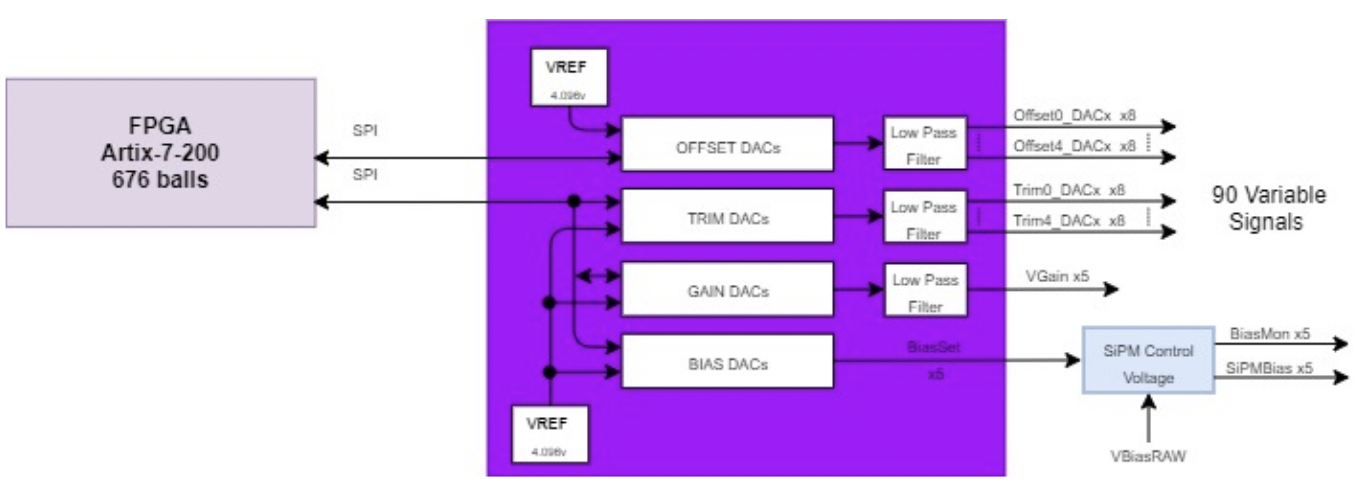
\includegraphics[width=.8\textwidth,trim=30 110 0 0,clip]{Images/BiasControl.png}
%\qquad
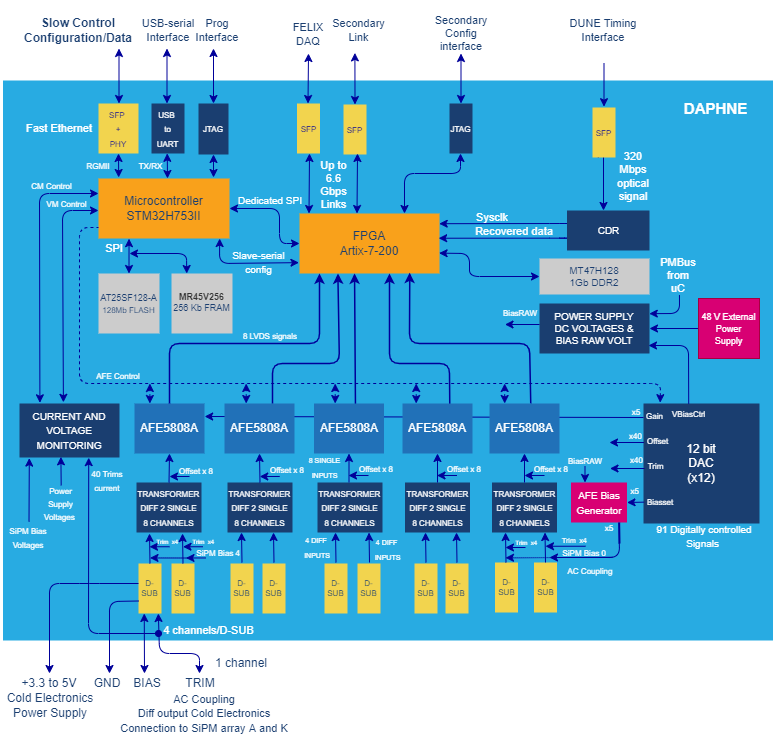
\includegraphics[width=1.\textwidth,origin=c,angle=0]{Images/Block_Diagram_DAPHNEV1_rev2.png}
% "\includegraphics" from the "graphicx" permits to crop (trim+clip)
% and rotate (angle) and image (and much more)
\caption{\label{fig:DAPHNEBlocksScheme} DAPHNE general scheme.}
\end{figure}

The first stage of signal conditioning is based on differential to single transformers. In this stage is, embedded the SiPMs bias voltage generator and control; more details are presented in section~\ref{sec:interfaces}  

The unipolar signals are digitized using the Analog Front End chips. There are 5 AFEs, eight channels each, for 40 channels. The AFEs are arrays of programmable active or passive impedances, a low noise amplification, an external voltage controller attenuator, a programmable gain amplification, a low pass filter, and 14 bits analog to digital converter. The control of all these elements is a task of the micro-controller embedded in DAPHNE.

The FPGA reads the digital data generated by the AFEs with a frequency of $62.5MHz$. In addition, the FPGA can select an event using an internal trigger and save the data that will be streamed by optical fibers to the DAQ system at a rate of $4.8Gbps$ using an external hardware and software protocol called FELIX (Cita) 


A more detailed description of the primary digital devices implemented in the DAPHNE board is presented in the following.

\subsubsection{AFE5808A}

The AFE5808A is an analog front-end (AFE) intended to be used in the digitization of analog signals \cite{afe5808a} for applications based on doppler effect. In the case of DAPHNE, its special characteristics fit according to experiment requirements, in few words 14 bits of data resolution, a sample rate of 62.5 Msps, embedded filtering techniques like Low pass filtering and high pass filtering, and finally a pre amplifier stage before digitizing the data.

There are two important interfaces to operate the AFE's

\begin{itemize}
\item Serial Peripheral Interface (SPI): Configuration via SPI. It is a standard serial interface used to write on configure registers, in order to enable, disable or configure the special characteristics present in this device. 

\item Data output: The interface it's an LVDS interface connected directly to the FPGA. Each AFE transmits to the FPGA a total of 10 LVDS signals; 8 LVDS signals corresponding to each analog input channel, 1 LVDS signal corresponding to the frame clock and 1 LVDS signal for the digital clock.
\end{itemize}

In the case of the AFE, DAPHNE uses 5 of such devices, eight channels each, for a total of 40 analog channels. 

The master clock input used for each AFE is provided by the FPGA that uses five clock generators coming from the timing interface.

\subsubsection{FPGA}

The FPGA is responsible of reading the digital data coming from the 5 Analog Front End's (AFE5808A). And the last one, is the responsible of processing 8 analog channels coming from the Cold Electronics(CE) as can be seen from the figure \ref{fig:DAPHNEBlocksScheme}.

The FPGA used on DAPHNE is the Xilinx Artix-7, model XC7A200T-676. The FPGA supports streaming data links of 4.8 Gbps together with a communication protocol specificated by CERN~\cite{Borga:2019rwr}. In order to implement the links the use of hte  GTP transceivers on-chip is mandatory and of course a couple of external SFP connectors in order to be independent of the used medium copper or optic fiber. 

A dedicated SPI interface with the microcontroller is available for different tasks. The AFE is controlled using an SPI interface, and the data reading is allowed using an LVDS interface using a SERDES-based module~\cite{IEEE_Ref2:understanding_LVDS}. Additional FPGA functions are clock generation for AFEs and internal FPGA temperature monitoring. 

\subsubsection{Microcontroller}

The STM32H753II Cortex-M7 implementing FreeRTOS, adding new support for this STM family, is the microcontroller device used on DAPHNE. The microcontroller is responsible for monitoring and slow control tasks. The DAPHNE board provides the voltages for the photosensors ganged together accountable for detecting the scintillation light; the DAPHNE microcontroller makes the voltages and current monitoring. For slow control, a fast Ethernet link through SFP is foreseen, but an USB/UART connection is available for debugging purposes.  

Internal no volatile and external volatile memory can be used for tasks like the permanent register of operational parameters (MAC addresses, IPs, etc.) and bitstream file upload to the FPGA. A JTAG interface for programming and debugging is available in DAPHNE.



 
 










\section{DAPHNE Interfaces}
\label{sec:interfaces}

The FEB has a direct connection with 4 subsystems: Cold Electronics, DAQ, Slow control and timing interface.

\subsection{Cold electronics}

The front-end-board DAPHNE and the so called Cold Electronics (CE) are intended to work together in order to detect and process photons collected by the X-ARAPUCA system. The CE consist of SiPM arrays and amplification electronics that are powered by the DAPHNE board.  

Each array consists of 48 SiPMs, where groups of 6 SiPMs are connected in parallel and 8 groups are ganged together, so in essences the 48 SiPMs are connected in parallel and constitutes an analog channel. The signals  are preconditioned using the so called cold amplifier which drives signals over a 100 $\Omega$  differential pair. The differential treatment of the signal between the cold electronics and DAPHNE is mandatory for the signal integrity. The constraints for this treatment are the distance to the cryostat, the impedance of the carrier cables and the frequency of the expected pulses. 
 
 DAPHNE is responsible for providing the bias voltage for the SiPM and a digitally controlled trim voltage to the cold electronics. Another digital voltage is used as a reference for the analog signal conversion, that voltage reference moves the reference into the AFE. All these signals are driven by DACs attached to the FPGA. 


\subsubsection{Bias voltage}

DAPHNE supplies a bias voltage (56V) to SiPMs arrays. The bias voltage is generated from a HV output of the power supply circuit; the voltage value is set by soldering a bridge on the specific point on the board. The figure~\ref{fig:DACsStage} shows the general scheme for the voltages generation (bias, trimming and offset). 

\begin{figure}[htbp]
\centering % \begin{center}/\end{center} takes some additional vertical space
%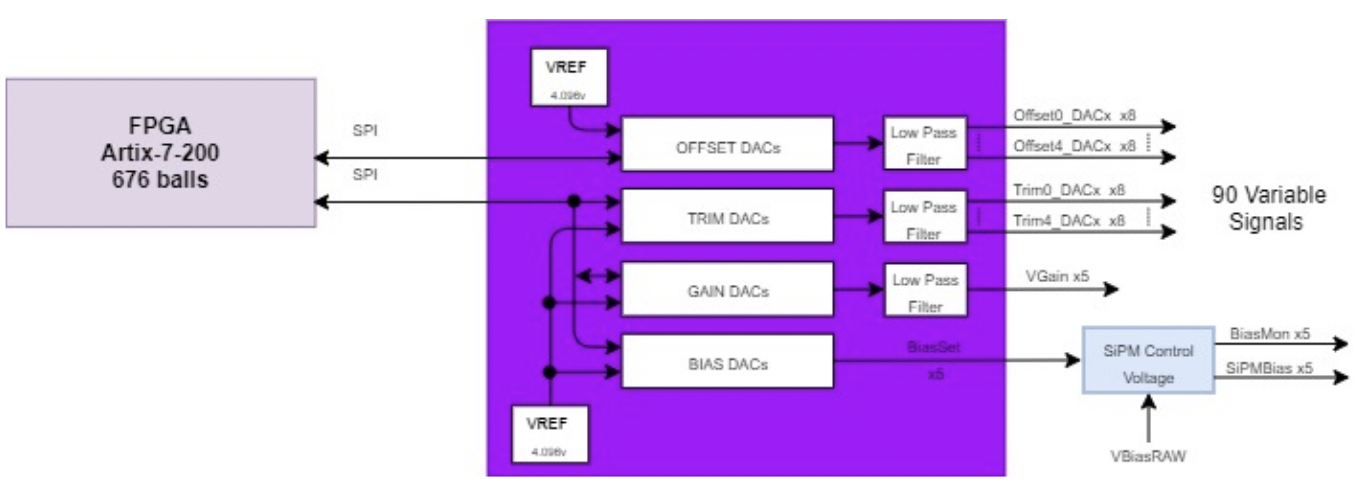
\includegraphics[width=.8\textwidth,trim=30 110 0 0,clip]{Images/BiasControl.png}
%\qquad
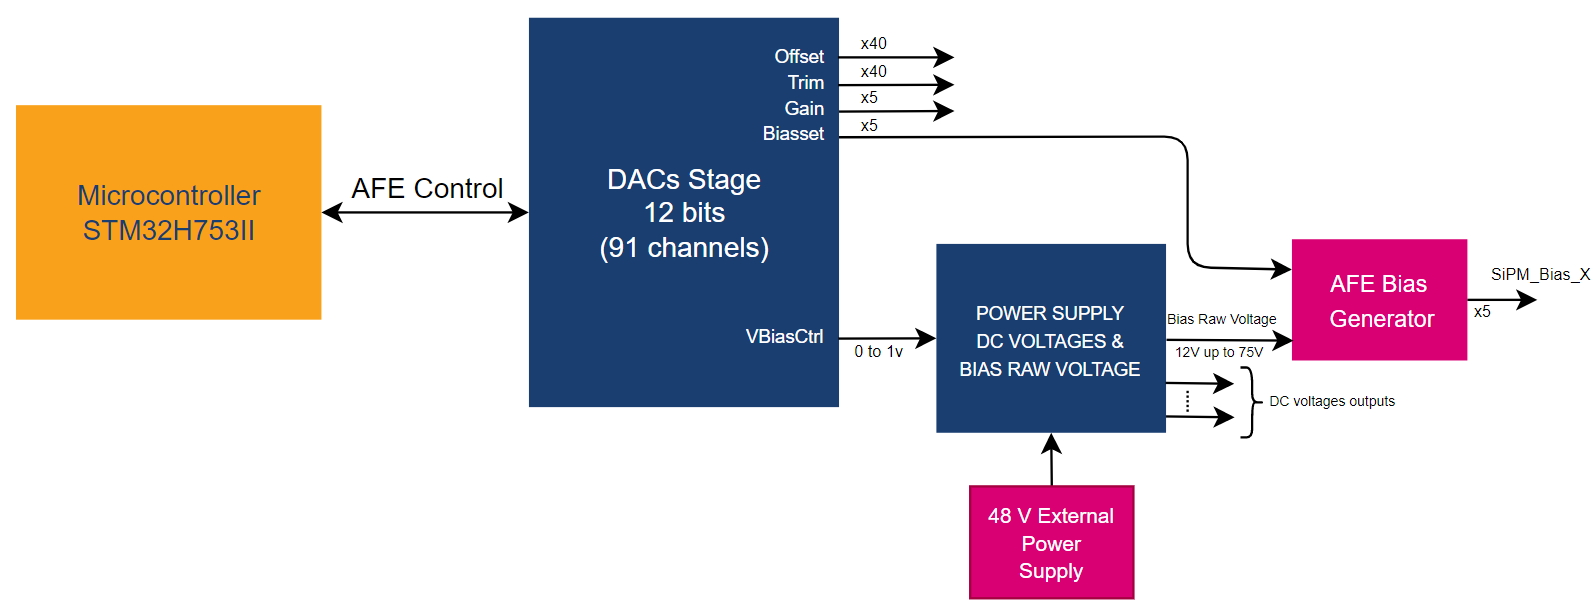
\includegraphics[width=.8\textwidth,origin=c,angle=0]{Images/DACsStage.png}
% "\includegraphics" from the "graphicx" permits to crop (trim+clip)
% and rotate (angle) and image (and much more)
\caption{\label{fig:DACsStage} Digitally-Controlled voltage generation.}
\end{figure}

This voltage is considered as a “Raw” voltage and is the source to generate the different bias signals to be connected to the CE via dedicated connectors.
Figure~\ref{fig:BiasCircuit} shows the circuit implemented for the SiPMBiasX signal generation; where X stays from 0 to 4, one for each AFE block. The circuit takes the Raw voltage (VBiasRaw) signal from the power supply and provides at the same time the BiasMonX signal, used to monitor the Bias by the ADC on the microcontroller. The design includes the BiasSetX signal, controlled by the FPGA using a GPIO pin. This allows DAPHNE to connect or disconnect the bias voltage as it is required.

\begin{figure}[htbp]
\centering % \begin{center}/\end{center} takes some additional vertical space
%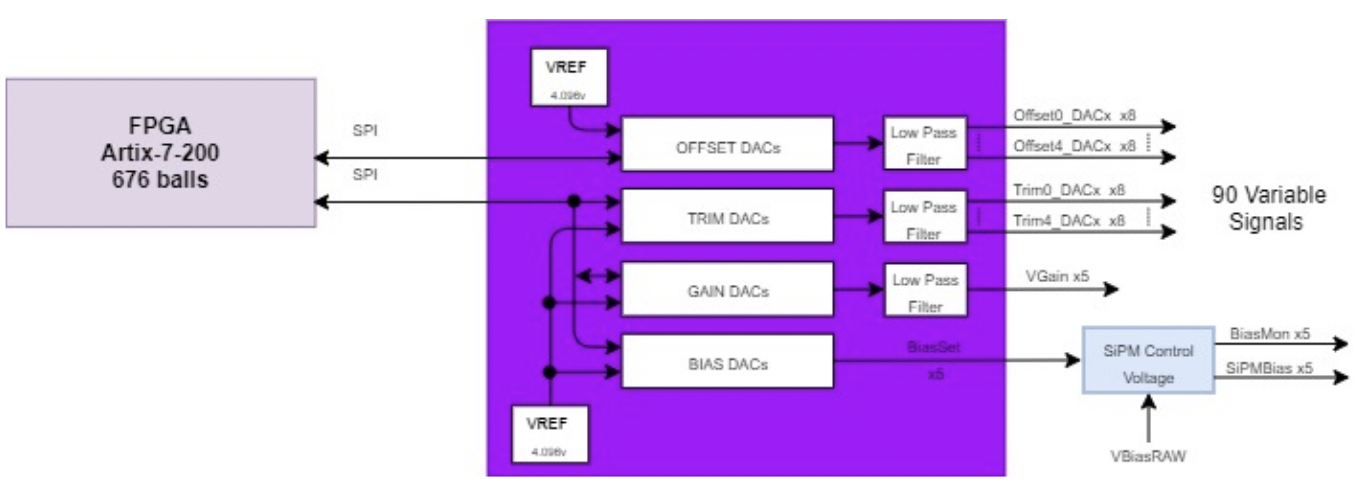
\includegraphics[width=.8\textwidth,trim=30 110 0 0,clip]{Images/BiasControl.png}
%\qquad
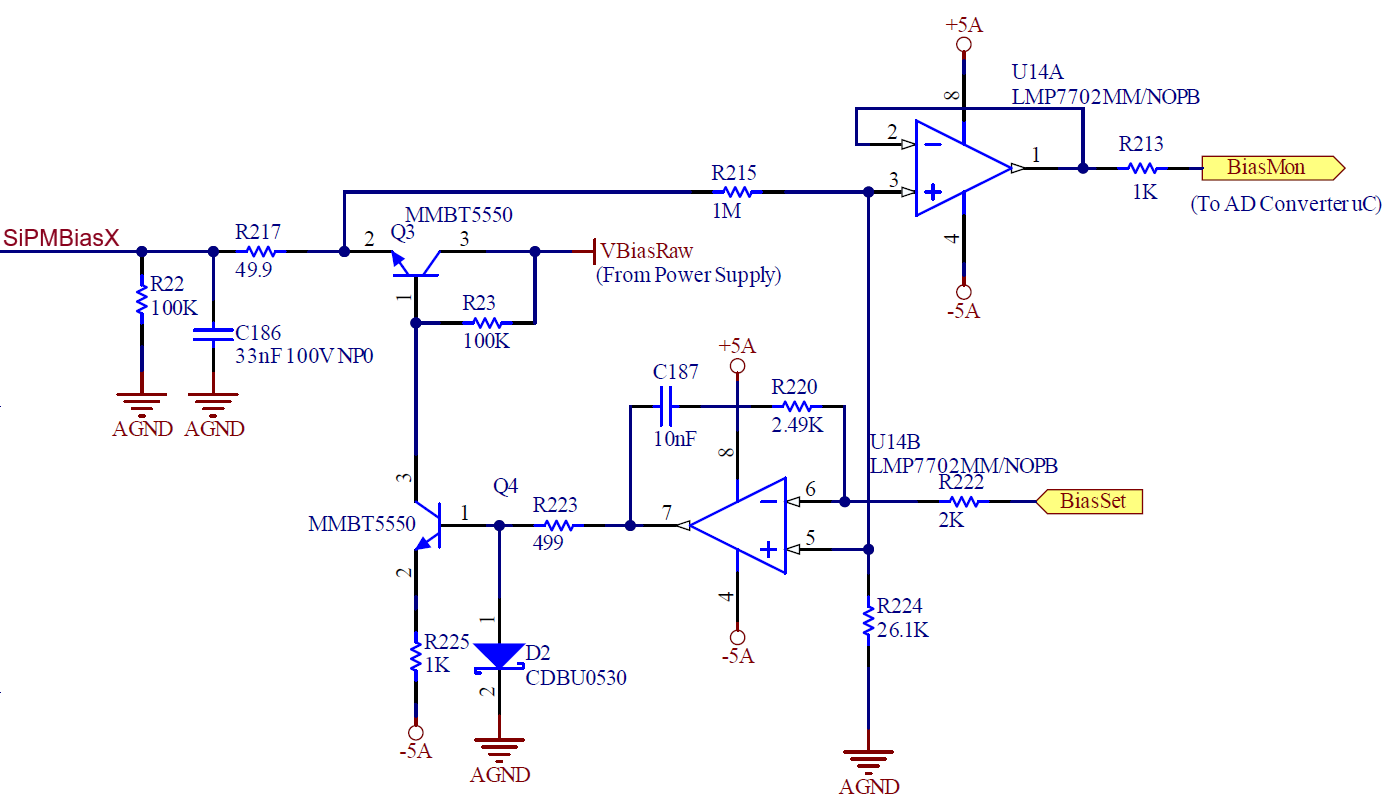
\includegraphics[width=.8\textwidth,origin=c,angle=0]{Images/BiasCircuit_v2.png}
% "\includegraphics" from the "graphicx" permits to crop (trim+clip)
% and rotate (angle) and image (and much more)
\caption{\label{fig:BiasCircuit} Bias voltage and monitoring circuit.}
\end{figure}

\subsubsection{Trimming voltage}

DAPHNE supports 40 trimming voltages, one for each channel. This voltage is variable from 0 to 4.096 V by using 5 AD5328 DAC devices. 

Figure~\ref{fig:TrimmCircuit} shows the different stages of one Trimming voltage generation, in this TRIM2\_DAC0. In this case, DAC2\_0 is a signal generated for the DAC, controlled by a SPI supported by the FPGA. Then, the signal is connected to a LMP7704 op-amp, to generate the TRIM2\_DAC0 signal. that is finally connected to the corresponding pin on the CE interface and to the monitoring interface.

\begin{figure}[htbp]
\centering % \begin{center}/\end{center} takes some additional vertical space
%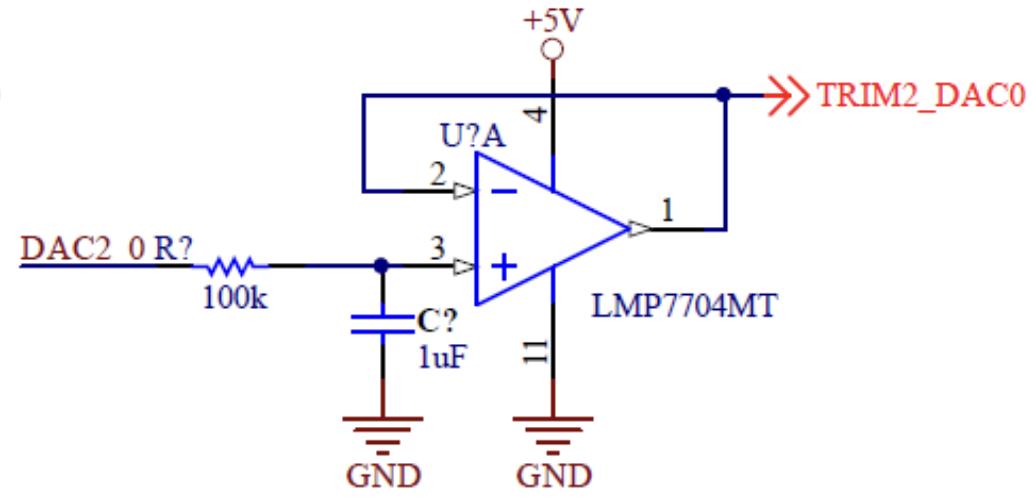
\includegraphics[width=.8\textwidth,trim=30 110 0 0,clip]{Images/TrimmCircuit.png}
%\qquad
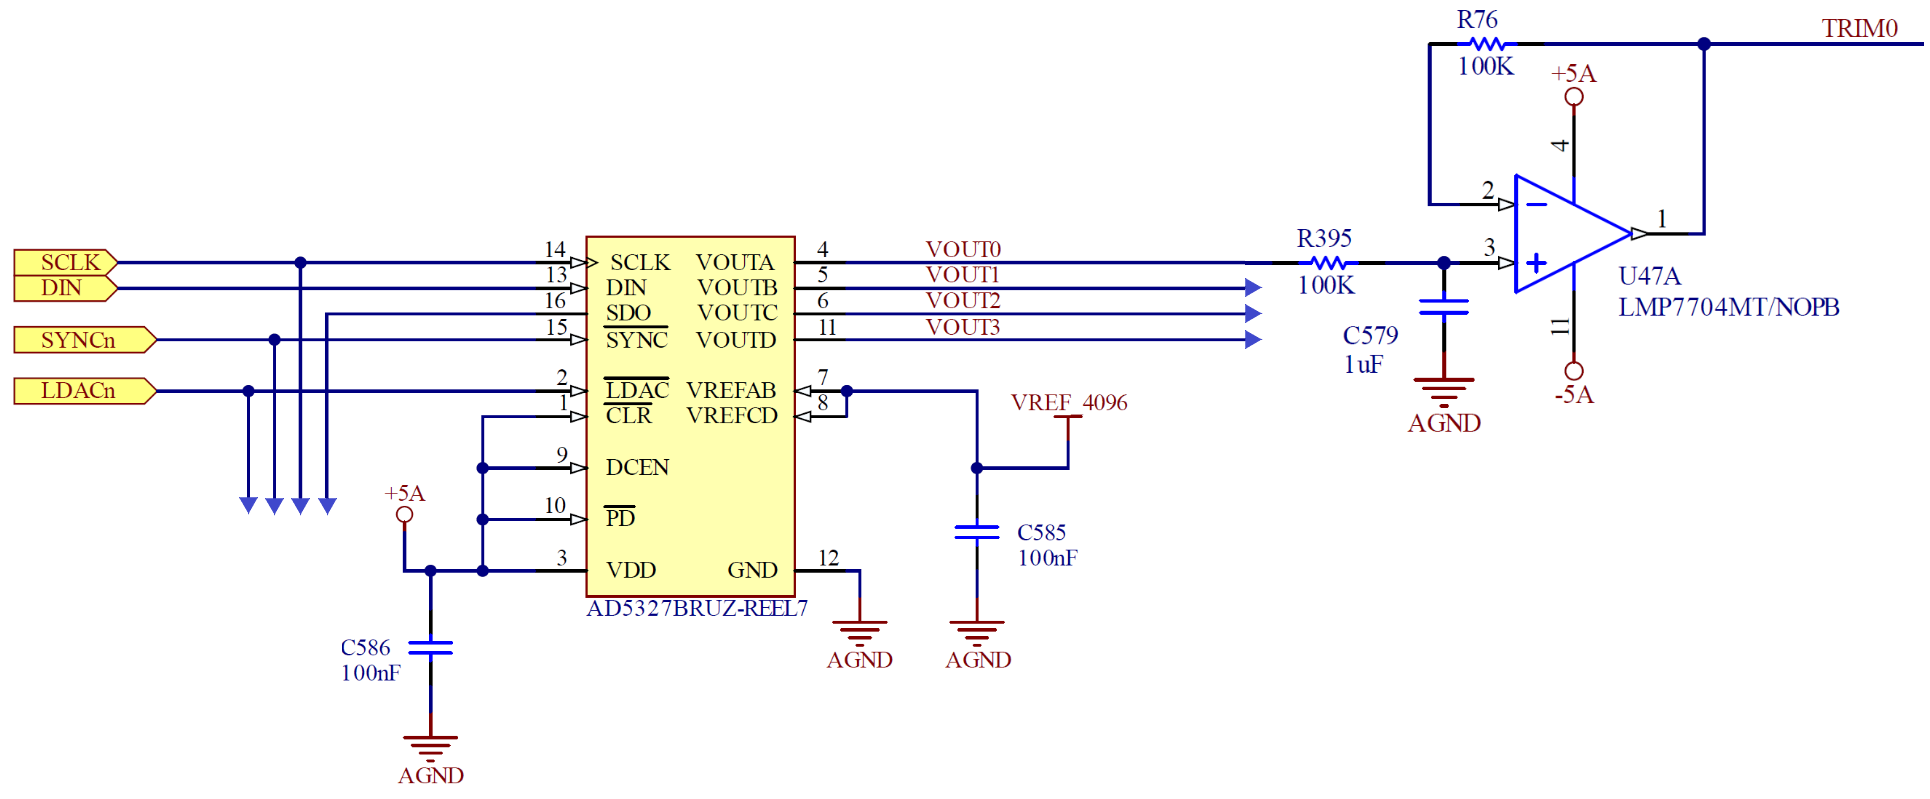
\includegraphics[width=.8\textwidth,origin=c,angle=0]{Images/TRIMCircuit_v2.png}
% "\includegraphics" from the "graphicx" permits to crop (trim+clip)
% and rotate (angle) and image (and much more)
\caption{\label{fig:TrimmCircuit} Trimming voltage generation circuit.}
\end{figure}

\subsubsection{Offset voltage}

An offset voltage is intended to generate a shift on the AFE input, required for analog to digital conversion. The scheme is the same as used for the trimming voltage, except that it does not use an op-amp stage to generate the signal after the DAC output.

The function of the offset voltage is shifting the signal to generate a behavior similar to a bipolar signal, but taking into account that the signal on the AFE input is unipolar, coming from the transformer that performs the differential to single conversion. This feature is one of the main differences between DAPHNE and the Mu2e board, because in the original design (Mu2e) the input is bipolar given the nature of the experiment and the AFE is configured to work with this kind of signals and in this case the by default configuration implies a DC-offset correction. 
If the PDS signals, that are unipolar are connected to the AFE in the same way of Mu2e, the result is that the analog conversion is performed only for the half of the range of the device and it is not effective to use a offset to force the AFE to convert in the entire range, because this offset would be eliminated for the DC-offset correction circuit.

During the DAPHNE design, it was found that it is possible disabling the DC-offset correction circuit, allowing the implementation of the offset shift for the unipolar signals and uses the AFE in the full conversion range in this way. 

\subsubsection{Cold electronics voltage}

 For the cold electronics voltage it used a +3V. To generate this voltage both a buck converter, LTC3624, and linear regulator, TPS7A701, are used. The buck converter will take +5.5V coming from the power transformer and convert it into +3.3V. The +3.3V will not be used for any other part of the board or FPGA. The linear regulator will then convert the voltage to +3V. Both the LTC3624 and TPS7A701 are adjustable so if a different cold electronics voltage was decided upon other than +3V then it could done by changing feed back resistors.

\subsubsection{Current and voltage monitoring}

DAPHNE is also responsible for the monitoring of currents and voltages delivered to each channel. There are 2 kind of signals to be monitored:

\begin{itemize}
  \item Voltages from the power supply
\item Bias and trimming voltage, with current monitoring
\end{itemize}
The monitoring is implemented by 2 separated ADCs with different resolutions:
\begin{itemize}
    \item Internal ADC on the STM32 microcontroller, which monitor Bias voltages (BiasMonX signals) and power supply voltages
\item ADC ADS1259, one-channel, delta-sigma, 24 bit, 14.4 Ksps for monitoring og trimming voltages %(DAx and DBx signals, referred to the figure 13)
\end{itemize}

In the case of the power supplies voltages, the interest is to have information about the state of the power supply and generates the corresponding alarms/flags, as well as initiate the required control actions in the case of an abnormal situation. Bias voltages are monitored with a low precision using the microcontroller ADC, taking into account that the bias generation is considered stable from the power supply. For the trimming voltage, it requires a better resolution for that reason DAPHNE has a high-resolution and high-performance ADC dedicated for this task. The implemented scheme to monitor the 40 trimming voltages includes a 2-stage analog-multiplexer based on ADG1609 IC and a single to differential conversion by using PGA280 amplifier, in order to generate the required differential signal for the ADS1259 ADC, as shown in figure~\ref{fig:CurrentandVoltageMonitoring}

\begin{figure}[htbp]
\centering % \begin{center}/\end{center} takes some additional vertical space
%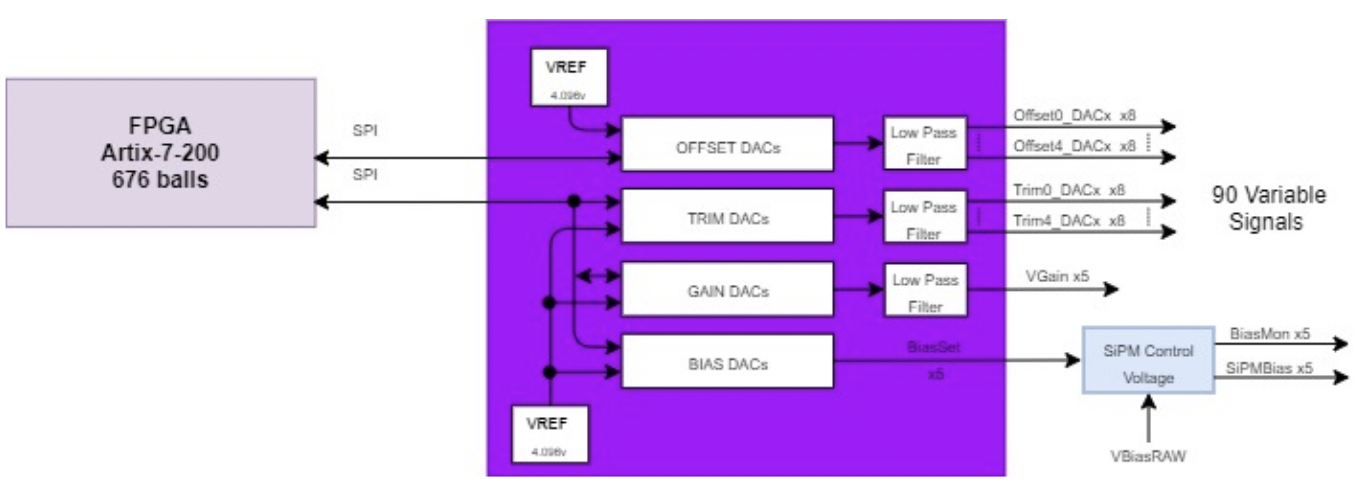
\includegraphics[width=.8\textwidth,trim=30 110 0 0,clip]{Images/BiasControl.png}
%\qquad
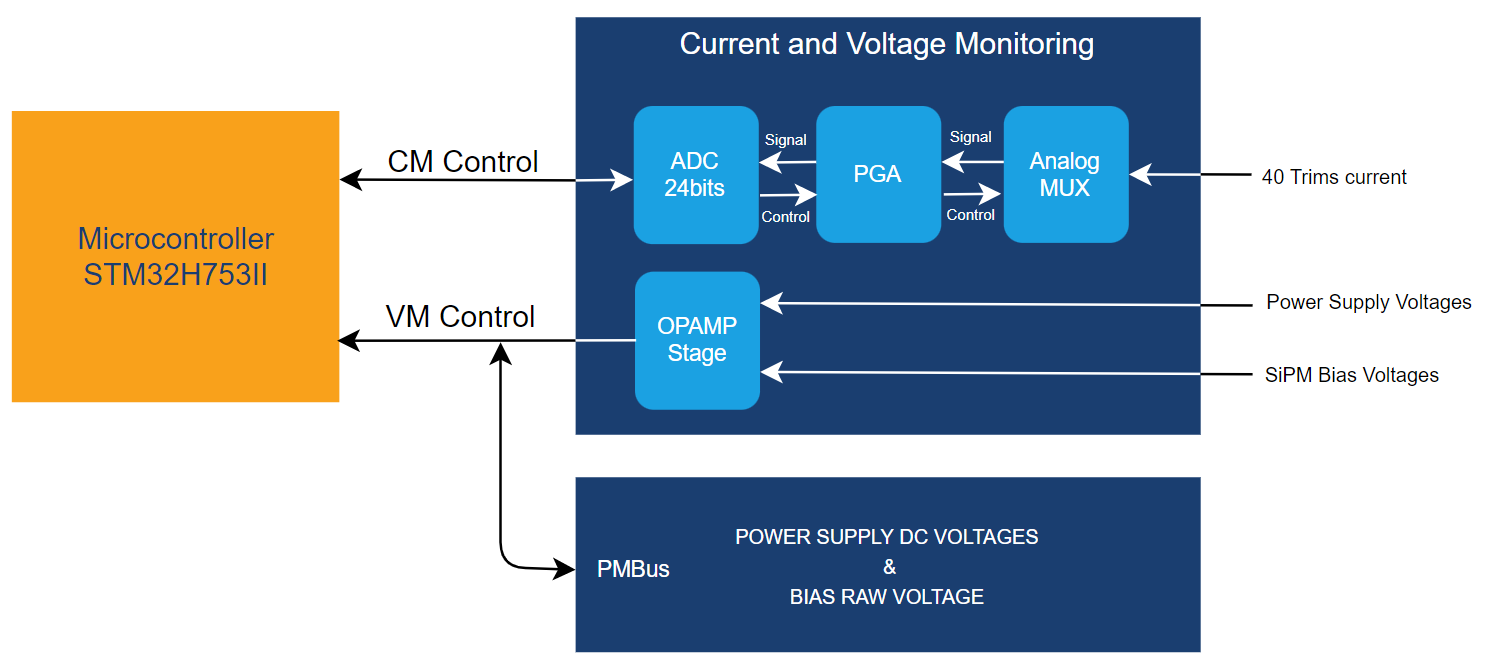
\includegraphics[width=.8\textwidth,origin=c,angle=0]{Images/CurrentandVoltageMonitoringV2.png}
% "\includegraphics" from the "graphicx" permits to crop (trim+clip)
% and rotate (angle) and image (and much more)
\caption{\label{fig:CurrentandVoltageMonitoring} Current and voltage monitoring.}
\end{figure}


%The digitization module consist of a differential to single converter, the AFE, and a readout control interface.  

\subsection{Slow control }

The main function of this interface is supporting slow control commands to be finally executed for the FPGA or the uC, depending on the peripherals to be controlled. The slow control consists of a fast ethernet connection controlled by the ST microcontroller, that uses a chain with a Wiznet chip and a PHY. The output of the link is a SFP transceiver, allowing optical fiber, RJ45 and a TCP/IP support.
The interface should handle flags in the power requirements of the board, allows monitoring of the XADCs on the FPGA and the General Error Handling of the FEB and Cold Electronics. 

The microcontroller communicates to the Wiznet via parallel interface, sending the required byte to be transmitted. The Wiznet supports the Fast Ethernet signaling and is connected to the PHY with optical fiber support. Finally, the PHY is connected to a SFP connector, intended to be used as a receptacle for specific transceivers, for example optical fiber or RJ-45. At the same time, there is a parallel interface connecting the FPGA and the microcontroller. The main source of data is the FPGA, that controls the data streaming from the AFE/ADC and eventually is necessary to communicate data through the Fast Ethernet Interface for debugging purposes. 

The FEB implements a server where a register matrix is refreshed in the microcontroller and in the FPGA. An error handling protocol is designed.

\subsection{DAQ}

One of the most important task that DAPHNE is required to accomplish is the communication of the signals generated by the PDS inside of the cryostat to the outside world. DAPHNE counts on two SFP transceivers for data streaming. This interface is supported by the GTP transceiver on the FPGA and are 6.6Gb/s capable in streaming mode. This special module allows DAPHNE to have a direct connection to an SFP connector. DAPHNE has 2 GTP connections, each one with a SFP connector including SFP cage, allowing the connection of any compatible SFP transceiver. In this case the purpose is connecting an optical fiber transceiver. Each SFP connector includes an I2C interface for control and configuration, connected to FPGA.

Both GTP Transceivers use a dedicated clock signal based on a crystal. The exact frequency of this crystal should be defined depending on the Full-mode specification and the adaptation to the half of the maximum rate proposed to operate on DAPHNE. The operation of this interface depends on the digital module implemented on the FPGA.

\subsection{Timing Recovery CDR}
The DAPHNE CDR module is based on the SoLiD CDR module developed at the University of Bristol~\cite{Arnold_2017}. The DUNE DAQ system provides a system clock of 62.5MHz for DAPHNE that is connected at the CDR port (Optical fiber). The module has an SFP connector for optical fiber support by using a transceiver. The signal is connected to an ADC2814 Clock and data recovery chip, which provides 2 separated data and clock signal. The data signal is connected to the FPGA in order to be used in the appropriate modules. The SFP connection has a dedicated i2c interface connected to the FPGA, used to control and monitor the interface.

The recovered clock signal is connected to a clock generator block, which includes a PLL, a low-pass filter, and a controlled oscillator. This block generates a continuous  clock signal depending on the Timing Interface input and the clock generator. The design includes the capability of continuing working even if the Timing Interface is disconnected. The CDR chip can detect the loss of the external signal and there is a flag for the control module. 

\subsection{LEMO connectors}

DAPHNE has 2 LEMO connectors intended to be used as external triggering and timing signals, in this case 1 input and 1 output. These connectors are directly connected clock capable pins on the FPGA and should be included in the gate structure implemented on the Artix-7.


\subsubsection{LEMO input} DAPHNE is prepared to work with an external clock input source at the LEMO connection. This connection will be used during the tests in absence of a system triggering clock, or with different rates at the streaming output.

\subsubsection{LEMO output}
The LEMO output allows us to sync other modules sharing the clock of the FPGA. It could be the LEMO input clock or the one of the inner programmable clock on the FPGA. A control loop can be runned to check the clock integrity of some modules or signals

\section{DAPHNE Firmware}
\label{sec:firmware}

Each DAPHNE board has 8 AFE's for a total of 40 analog channels, the analog to digital conversion resolution is 14 bits,  and the sampling rate is 62.5MSPS. %The reading out of the expected data volume implies the use of dedicated firmware involving self-trigger scheme and zero suppression algorithms.  
A differential data bus is used in order to read all the digitized signals, the DDR data format can be seen in figure~\ref{fig:Datos_AFE}.

\begin{figure}
\centering % \begin{center}/\end{center} takes some additional vertical space
%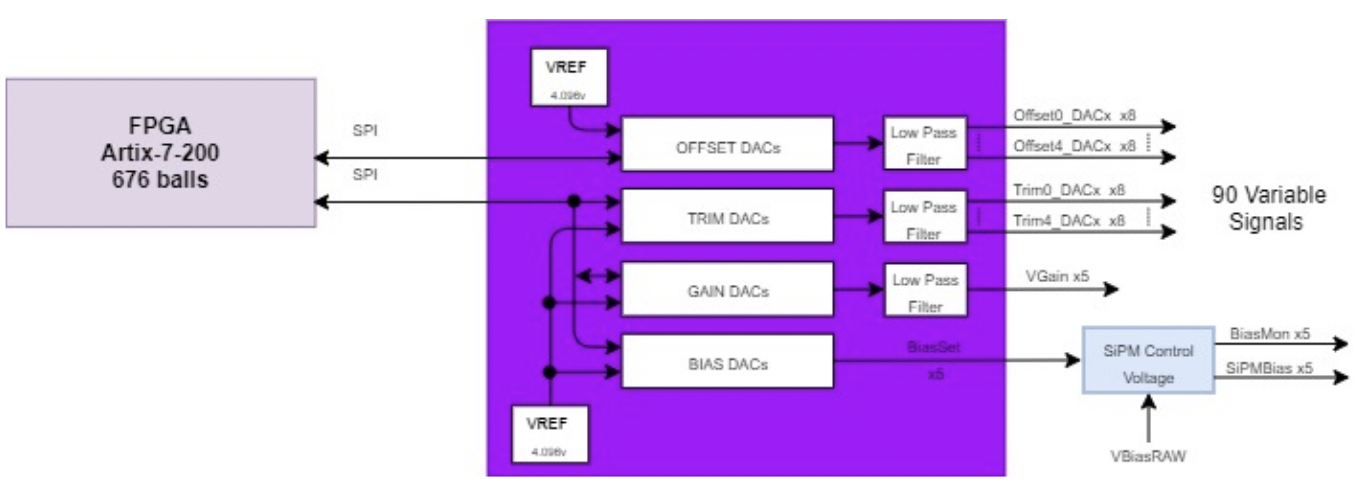
\includegraphics[width=.8\textwidth,trim=30 110 0 0,clip]{Images/BiasControl.png}
%\qquad
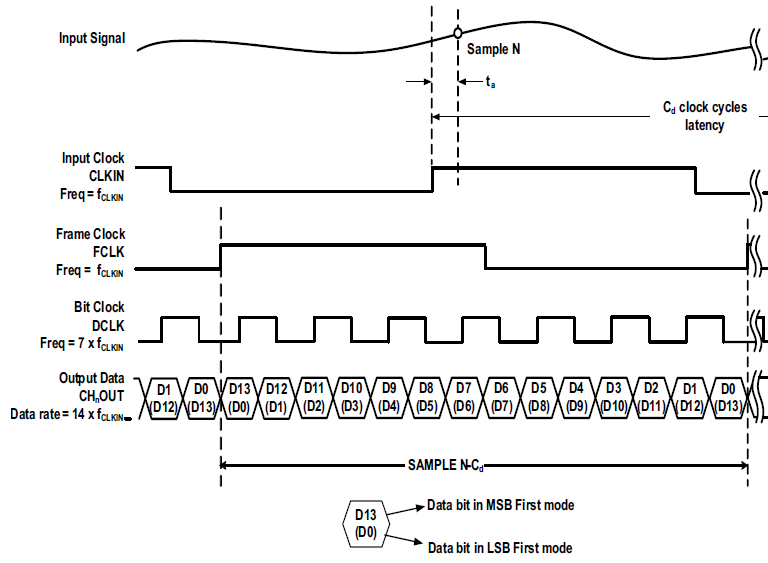
\includegraphics[scale=0.7,origin=c,angle=0]{Images/serial_data_AFE.png}
% "\includegraphics" from the "graphicx" permits to crop (trim+clip)
% and rotate (angle) and image (and much more)
\caption{\label{fig:Datos_AFE} Scheme of serial data reading on an AFE.}
\end{figure}

In order to have a proper DDR reading, the alignment of the digital clock with the center of the data bits is a must, and there are 2 common methods to do it. 

The first one, uses a PLL with multi-phase outputs. In this method, the FPGA uses the clock delivered by the AFE, pass it through a PLL primitive to align the phase of the data clock with the center of the data bits,  to finally obtain a simultaneous alignment of the 8 channels with the digital clock. 

In the second method, discrete time delays are applied to each data signal, these are added by a dedicated FPGA primitive called IDELAY. One should add as many delays are necessary to align each center of the data bit, with the digital clock that comes from the AFE.

Once the data bit is aligned with the bit clock, another process shall be made, in order to align the 14 bit frame with the frame clock. This process is named bitslip, and is an embedded functionality of the used HDL primitive called ISERDES.\cite{XILINX_Ref1:XAPP585,limitinganalog,semiconductor2009high}

At the moment of writing this paper both reading methods are implemented and a test of the performance of each is undergoing.


\subsection{Microcontroller Firmware}

The microcontroller performs the Slow Control, which is the interface of configuration and fitting of the different digitization parameters through the peripherals that carry out the conditioning, in addition to monitoring some variables of the DAPHNE board.

The microcontroller was configured to use Real Time Operating Systems (RTOS) to perform the activities proposed in the Slow Control. RTOS allows to efficiently distribute the tasks to be performed, redundantly evaluate the monitoring variables and avoid the microcontroller to inter in a halted state. The Figure \ref{fig:FirmwareMCU} shows the configuration scheme of the microcontroller.

\begin{figure}[htbp]
\centering % \begin{center}/\end{center} takes some additional vertical space
%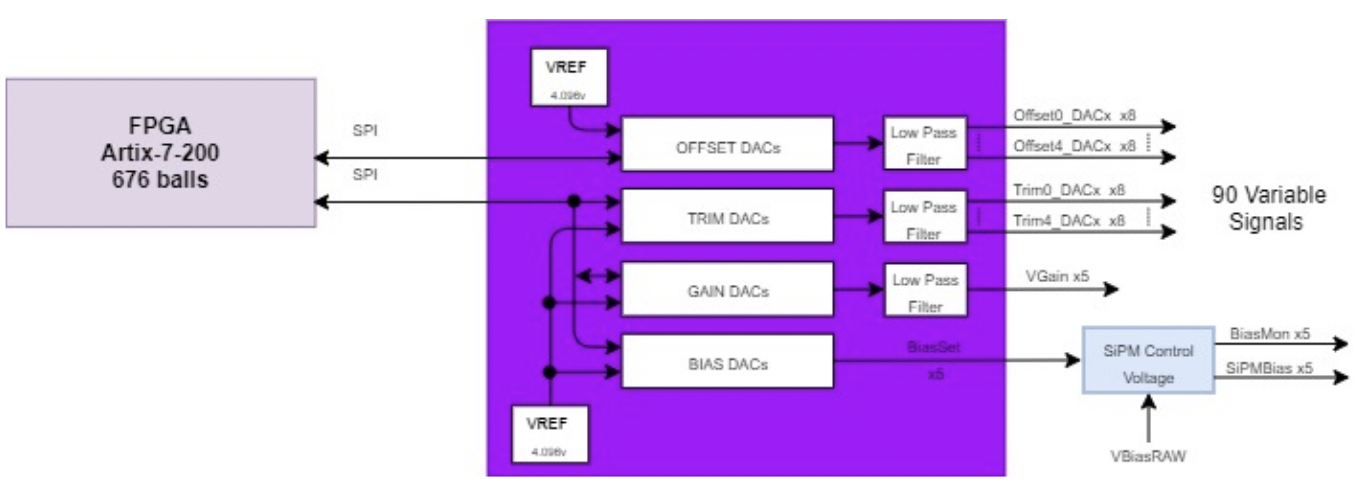
\includegraphics[width=.8\textwidth,trim=30 110 0 0,clip]{Images/BiasControl.png}
%\qquad
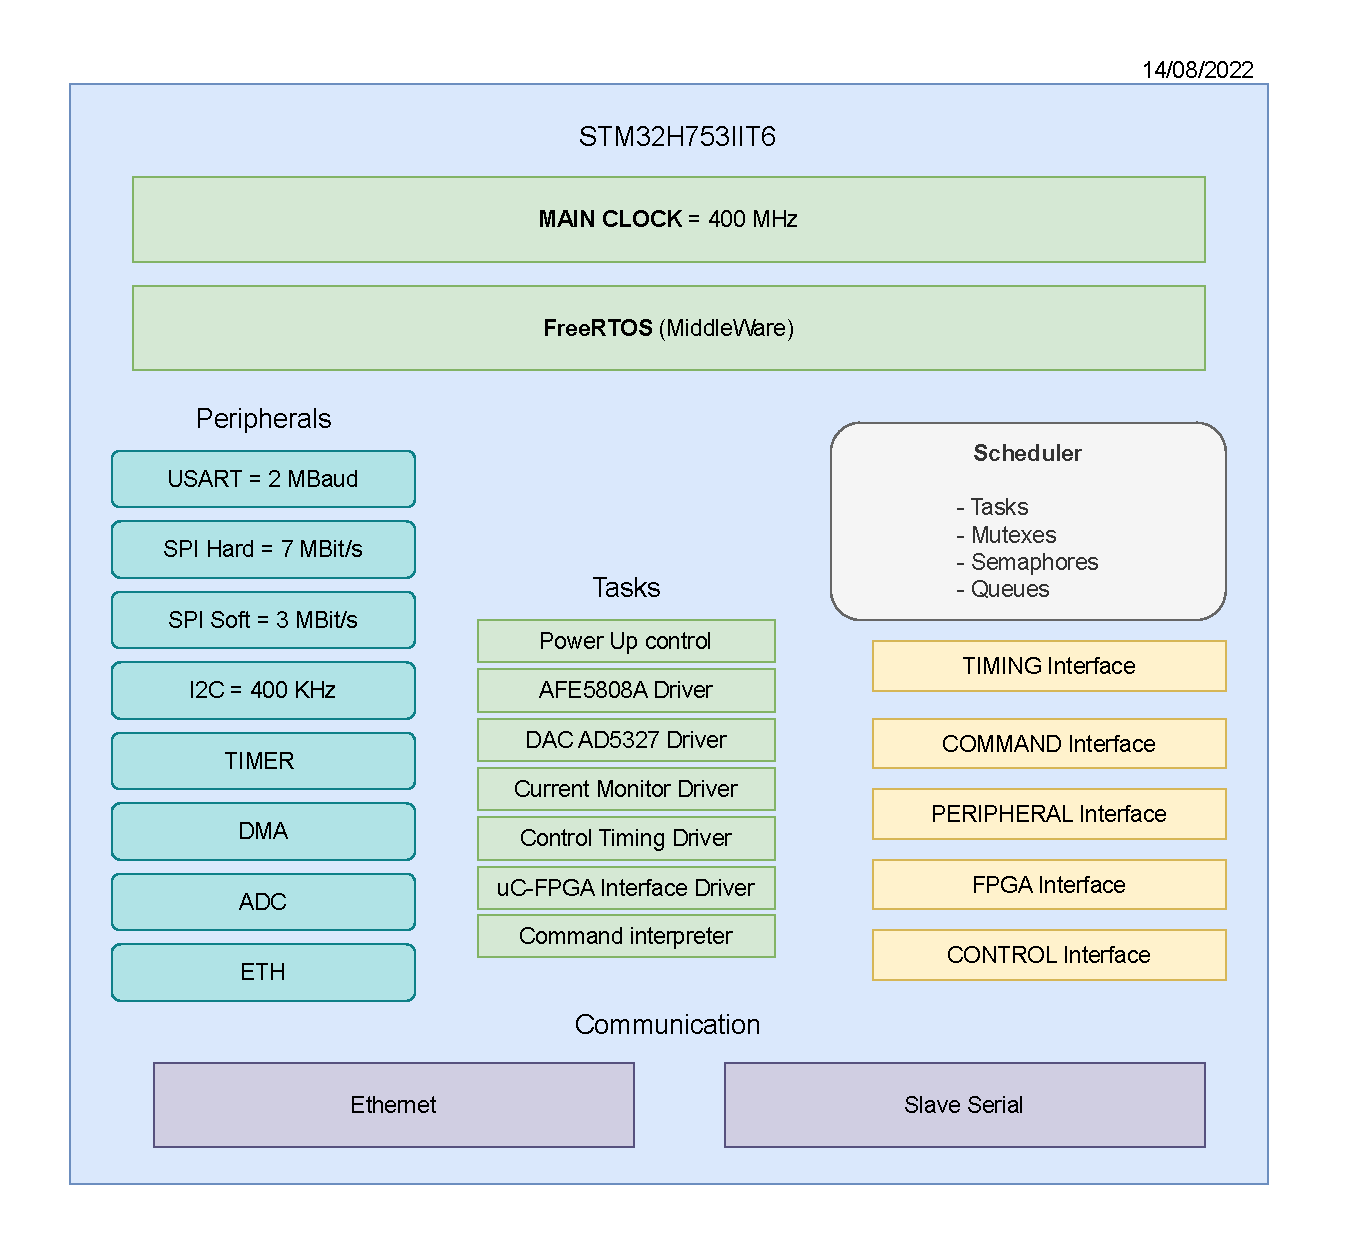
\includegraphics[width=0.8\textwidth,origin=c,angle=0]{Images/FirmwareMCU.pdf}
% "\includegraphics" from the "graphicx" permits to crop (trim+clip)
% and rotate (angle) and image (and much more)
\caption{\label{fig:FirmwareMCU} Microcontroller configuration scheme.}
\end{figure}

This diagram shows the configuration of the different peripherals of the microcontroller highlighted in aqua. In green, the distribution of tasks handled by the RTOS are highlighted. In yellow are presented the interfaces implemented to control and configure DAPHNE. Finally, the implemented communication interfaces highlighted in purple are presented.

This section describes the different stages that compose the firmware implemented in the microcontroller to perform the peripheral control, configuration and monitoring. 


\subsection{FreeRTOS (MiddleWare)}

FreeRTOS is a real-time operating system developed mainly for embedded devices, microcontrollers and small microprocessors. FreeRTOS has been adopted and implemented on more than 35 platforms including ARM and it is currently distributed under the MIT license. FreeRTOS implements methods for multiple threads, mutexes, semaphores, queues and software timers. It allows thread priority to be determined and device-specific interruptions to be handled. FreeRTOS also has a thread marking system that switches tasks according to their priority in a round-robin scheduling scheme \cite{freertos}. All these characteristics make it ideal for the implementation of highly complex and multitasking software such as that required in Slow Control for DAPHNE.


The firmware for DAPHNE was designed to perform six main tasks: Peripheral initialization, internal board monitoring, peripheral configuration and control, command interface, FPGA Bitstream load management, and Open Platform Communications Unified Architecture (OPC-UA) Server. Each of these tasks uses hardware and memory resources of the microcontroller that must be shared. Therefore this management with FreeRTOS allows the use of signaling through mutexes, semaphores, and its scheduler to handle the execution of the different tasks as multiple threads to avoid a possible collision.


\subsection{Peripheral initialization}

This task performs the initialization of all the peripherals to which the microcontroller has access and that must have a specific initialization sequence to guarantee the correct functioning of DAPHNE. Figure \ref{fig:InitPeriTask} shows the operating diagram for the initial configuration of the peripherals.

\begin{figure}[htbp]
\centering % \begin{center}/\end{center} takes some additional vertical space
%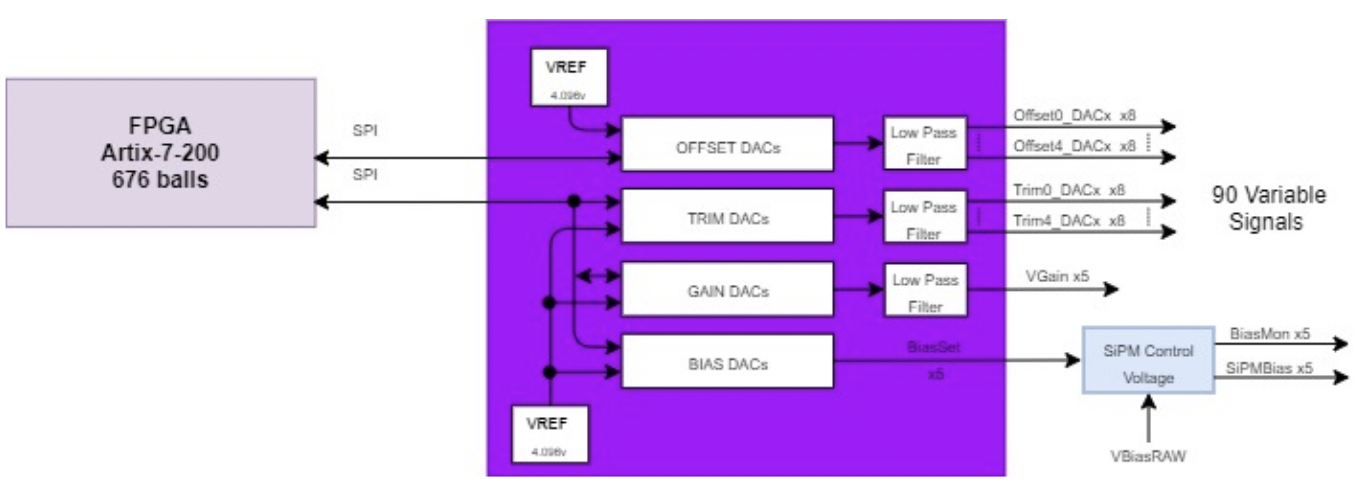
\includegraphics[width=.8\textwidth,trim=30 110 0 0,clip]{Images/BiasControl.png}
%\qquad
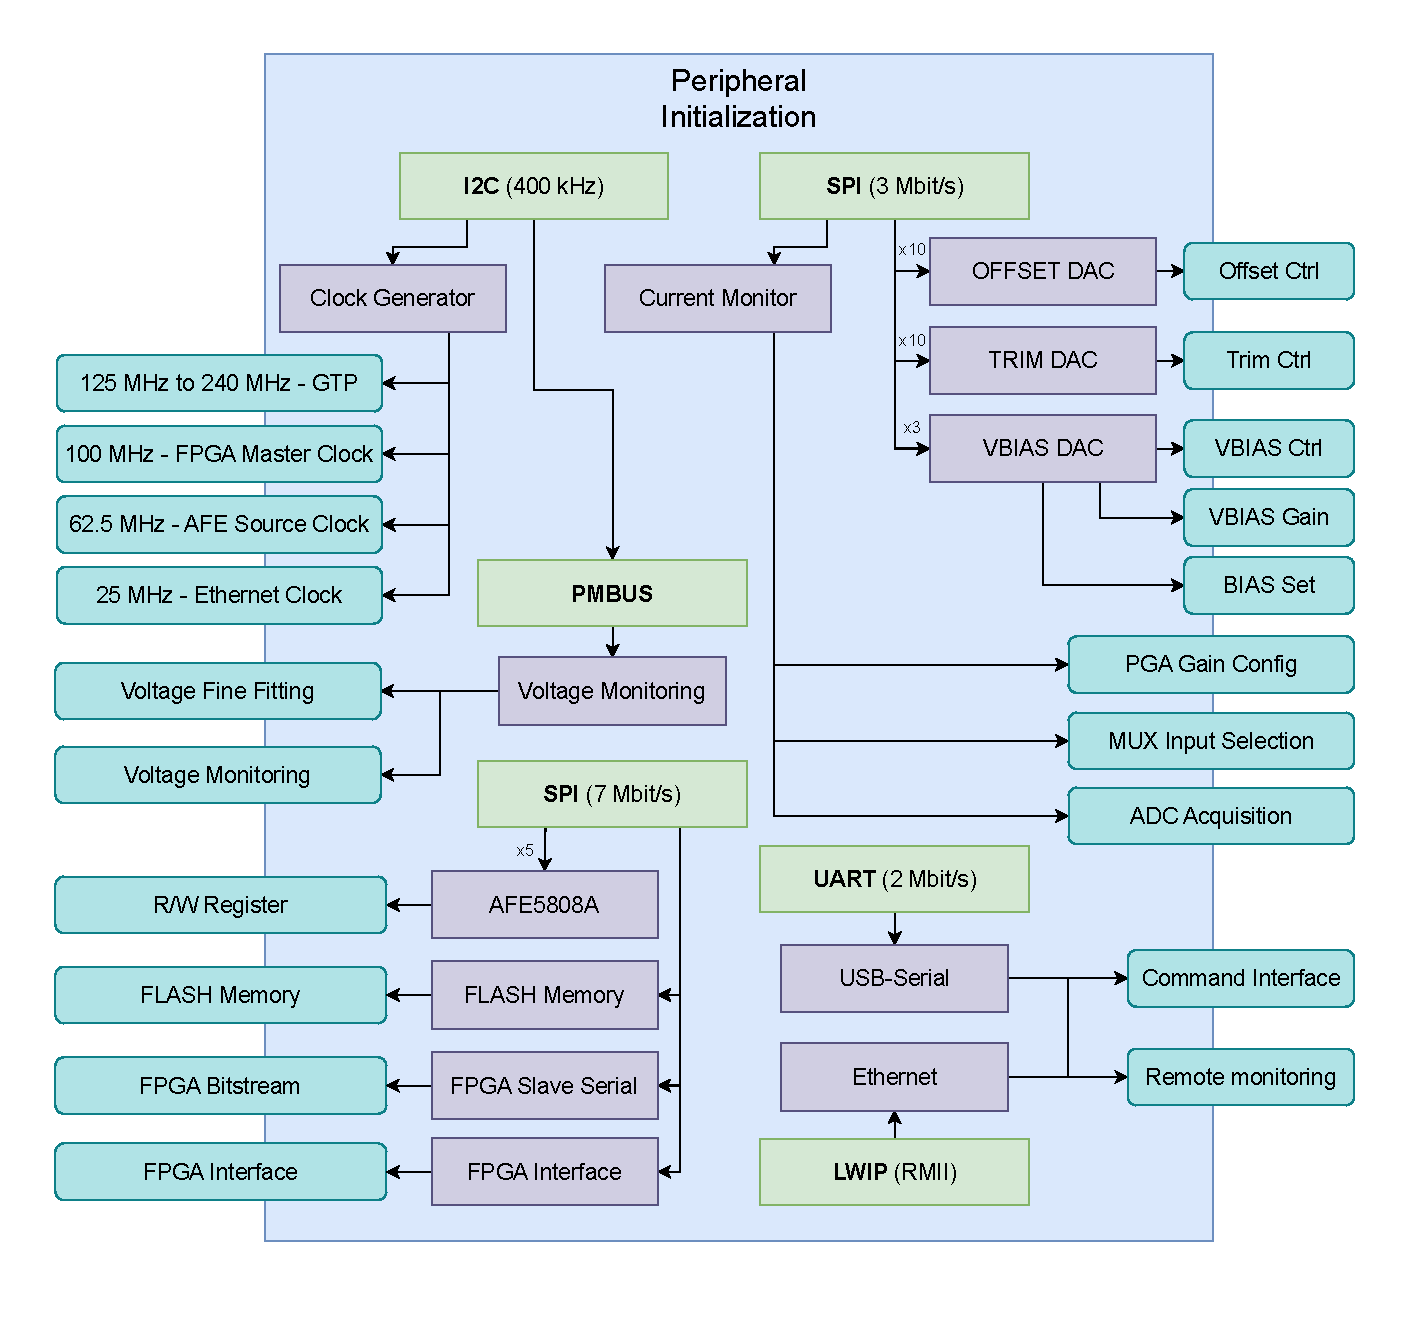
\includegraphics[width=0.9\textwidth,origin=c,angle=0]{Images/PeripheralInitTask.pdf}
% "\includegraphics" from the "graphicx" permits to crop (trim+clip)
% and rotate (angle) and image (and much more)
\caption{\label{fig:InitPeriTask} Peripheral initialization task scheme.}
\end{figure}

The first step in the configuration process is to configure the internal peripherals of the STM32H753IIT6 microcontroller \cite{stm32h7}. Once this configuration fits the requirements of each module, the initialization of the external peripherals is carried out through the writing of the internal memory registers to guarantee their operation in the desired mode.


\subsubsection{USART 2Mbit/s}

The Universal Serial Asynchronous Receiver Transmitter (USART) protocol was configured to be used at 2 Mbits/s with flow control by hardware. Also, the internal Interruption Service Routine (ISR) from the microcontroller was used to handle the data reception as events. All the information received through the USART module was handled by the Direct Memory Acces (DMA) module and stored in the FIFO structure of the RTOS Queue to prevent the collision in the use of memory resources of the microcontroller. The USART module aims to manage the Command Interface with a Host computer through a USB connection.


\subsubsection{SPI Hard 30Mbit/s 7Mbit/s and Soft 3Mbit/s}


One of the most useful features of the Serial Peripheral Interface (SPI) is the capability to connect multiple devices in the same communication bus. In this case, the microcontroller has six independent SPI modules which were used and distributed to the different peripherals. 

Two of them were used to control the AFE5808A at 7 Mbit/s to read and write the registers' memory and configure the different characteristics of these AFE modules. Also, to control the ADS5327BRUZ at 3 Mbit/s just to write the memory registers and control the voltage generated by each DAC in the subsystems (Trim DAC, Offset DAC, VBIAS DAC).

An SPI module was used to perform the Current Monitoring in the DAPHNE board, but also to control some AFE and DAC peripheral, sharing some hardware resources. This made it necessary to manage these resources through RTOS tasks separately. 

Also, an SPI module at 30 Mbit/s was used to control the FRAM and FLASH memory where some important configuration data is stored and the Bitstream for the FPGA respectively.

Finally, the other two SPI modules at 30 Mbit/s were used to implement a direct communication with the FPGA as a channel to configure or share some information between both processors and the other to load the Bitstream in the FPGA through the Slave Serial. 


\subsubsection{I2C 400kHz}

The Inter-Integrated Circuit (I2C) protocol allows connecting multiple devices in the same bus differentiated by their addresses. This module was configured with a 400 kHz clock signal to configure the Clock Generator and the PMBUS protocol to perform the Voltage Monitoring.

On the other hand, the PMBUS protocol allows to monitor the voltage generated by the voltage regulator and allows to fit the voltage value in a finer way.


\subsubsection{Ethernet}

The LwIP stack was used to configure the Ethernet module on the STM32H753IIT6 microcontroller. RMII was used as the peripheral configuration since it uses a reduced number of pins. High speed response was selected as the speed for the switching state of the pins associated with the Ethernet module.

As an important step in the configuration, it was necessary to enable the Memory Protection Unit (MPU) for the ICache and the DCache. Also, direct access to the microcontroller's D2RAM memory was defined. The PHY chip used in DAPHNE is the DP83620 which is a base 100 Mbit/s fiber optic transceiver \cite{dp83620}. The PHY receives the clock signal from the Clock Generator at 25 MHz.

The Ethernet was configured so that each DAPHNE had a unique MAC Address and a unique static IP, which can be configured from the command interface and is loaded from the FLASH memory when DAPHNE is started up.

In the application layer, the OPC-UA protocol was implemented in server mode to monitor some important variables of the board and to receive the commands that are then processed by the command interface.



\subsection{Board Monitoring}


The second task of the FreeRTOS is in charge of monitor peripheral functioning. This task executes the voltage monitoring, the current monitoring, and the Clocks Generation.

As was shown in Figure \ref{fig:InitPeriTask}, the voltage monitoring provides information about the state of the voltage power supply and the Bias and Trim voltage to inform the system about a possible risk of High power consumption that can affect the results of the experiment or damage the DAPHNE board, also with the current monitoring.

On the other hand, the Clock Generator produce four different clock signals:
 \begin{enumerate}
     \item GTP clock from 125 MHz to 240 MHz: This clock is configured by software through the command interface and is used to feed the GTP module.
     
     \item FPGA master clock at 100 MHz: This clock signal works as the master clock for the FPGA.
     
     \item AFEs source clock at 62.5 MHz: This clock is generated as a differential signal and it is directed to the FPGA where it is buffered to the clock fanout and distributed to the five AFEs separately.
     
     \item Ethernet clock at 25 MHz: This clock is used to feed the PHY chip.
     
 \end{enumerate}
 
Some of these clocks need to be synchronized to execute specific tasks like the alignment of the AFE's readout data and the Ethernet data transmission.


\subsection{Peripheral Configuration and Control}



\begin{figure}[htbp]
\centering % \begin{center}/\end{center} takes some additional vertical space
%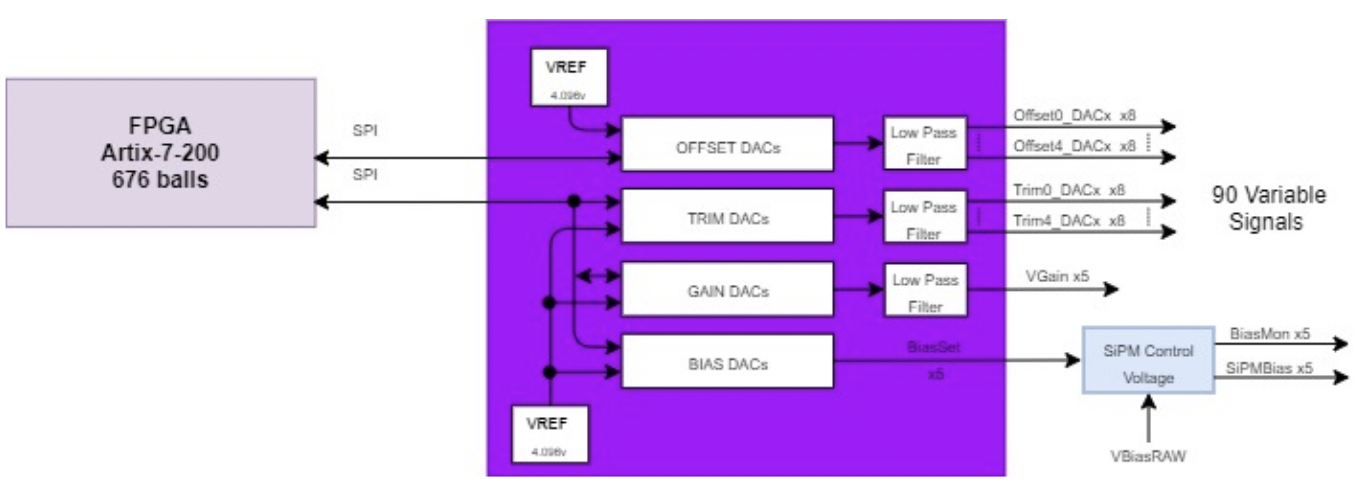
\includegraphics[width=.8\textwidth,trim=30 110 0 0,clip]{Images/BiasControl.png}
%\qquad
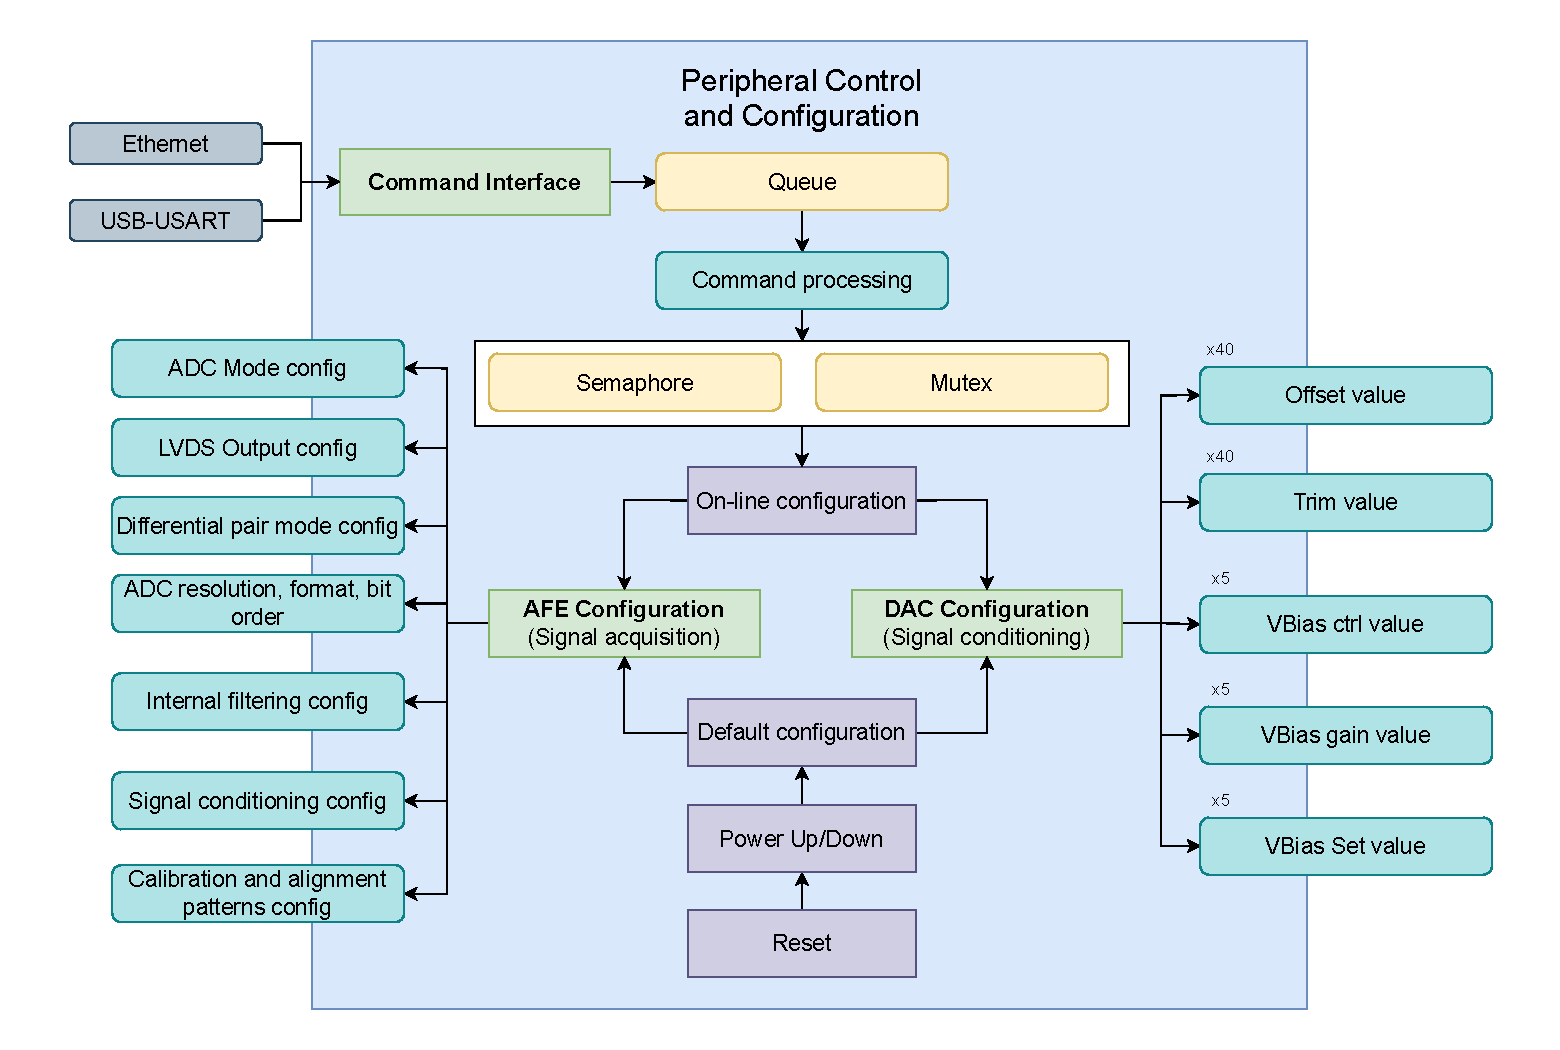
\includegraphics[width=0.9\textwidth,origin=c,angle=0]{Images/ControlTask.pdf}
% "\includegraphics" from the "graphicx" permits to crop (trim+clip)
% and rotate (angle) and image (and much more)
\caption{\label{fig:InitPeriTask} Control and configuration task scheme.}
\end{figure}





%Control de los diferentes perifericos para cambiar su configuracion en tiempo de ejecucion, esta tarea esta ligada con el command interface, y depende de la liberacion de recursos como QUEUEs, MUTEX, SEMAPHORES, 

%\subsubsection{Power Up control}

%Ajuste fino de los voltajes de los reguladores

%\subsubsection{AFE Configuration}

%COnfiguracion completa de los registros del AFE, tambien permite realizar la consulta de la configuracion actual 

%\subsubsection{DAC Driver}

%COnfiguracion y ajuste de los voltajes de salida de los DACs

%\subsubsection{Control Timing Driver}

%Control de los CLOCKs generados por el CDR

%\subsubsection{Current Monitor}

%Configuracion de las ganancias de los PGA, multiplexacion de las entradas para el monitoreo.



%\subsection{Command Interface}

%Interface de comandos que recibe los comandos para la ejecucion de difernetes acciones dentro del microcontrolador, los comandos pueden venir desde el USART o desde el OPC-UA a traves de ETH. los comandos son interpretados, gestioandos y direccionados principamnete a la tarea de configuracion y control de perifericos para ejecutar las acciones requeridas, una vez estas se han ejecutado, la interface de usuario envia una respuesta indicando el estado de la ejecucion.

%\subsubsection{Command interpreter}

%Explicar la estructura del command interpreter, y del command interface



%\subsection{FPGA Bitstream Load}

%Esta tarea se encarga de la comunicacion con la FPGA y con la memoria FRAM, almacenamiento del Bitstream, carga a la FPGA a alta velocidad a traves del Slave Serial, ademas de realizar streaming de datos a traves de una interface SPI hacia el microcontrolador de los datos recolectados a gran velocidad por los AFEs, datos previamente alineados en la FPGA

%\subsubsection{uC-FPGA Interface}

%Cpnexion SPI para gestion de comunicacion entre microcontrolador y FPGA

%\subsubsection{FRAM interface}

%Comuinicacion con la FRAM para almacenamiento y lectura del Bitstream de la FPGA

%\subsubsection{Slave Serial}

%Protocolo de envio del Bitstream hacia la FPGA, se implementa tambien un protocolo CRC para la verificacion de los datos enviados en el Bitstream




%\subsection{OPC-UA Server}

%Servidor OPC-UA para el monitoreo del estado de la tarjeta, consulta de las variables internas de DAPHNE, envio de comandos y recepcion de respuestas, todo gestionado a traves de este protocolo para acceder de manera remota y a traves de Ethernet a las diferentes tarjetas DAPHNE que componen el experimento de photodeteccion.

%\subsubsection{OPCUA}

%el OPC-UA permite gestionar la comunicaion con las diferentes tarjetas mediante las direcciones unicas que estas reciben por el protocolo Ethernet














\section{DAPHNE Data Sample}

\hl{Aqui se agregaran las figuras de los datos y muestras que se tomaron en las pruebas de los AFEs, tanto de las senales generadas por los AFEs para ver la sincronizacion como de algunas muestras de senales reales generadas por generadores de senales y adquiridas por DAPHNE.}

\begin{figure}[htbp]
\centering % \begin{center}/\end{center} takes some additional vertical space
%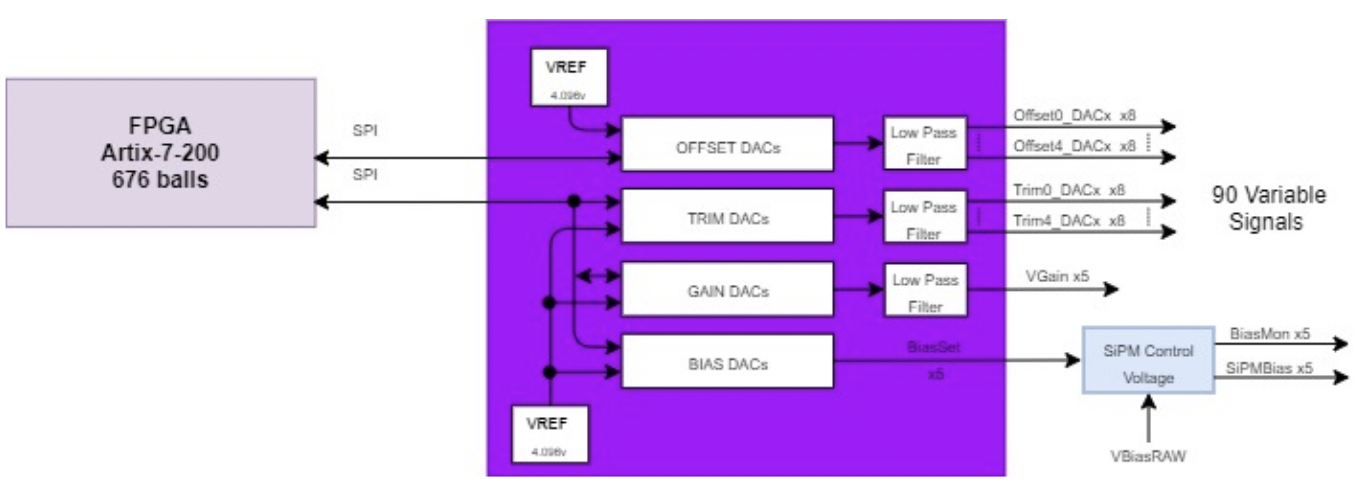
\includegraphics[width=.8\textwidth,trim=30 110 0 0,clip]{Images/BiasControl.png}
%\qquad
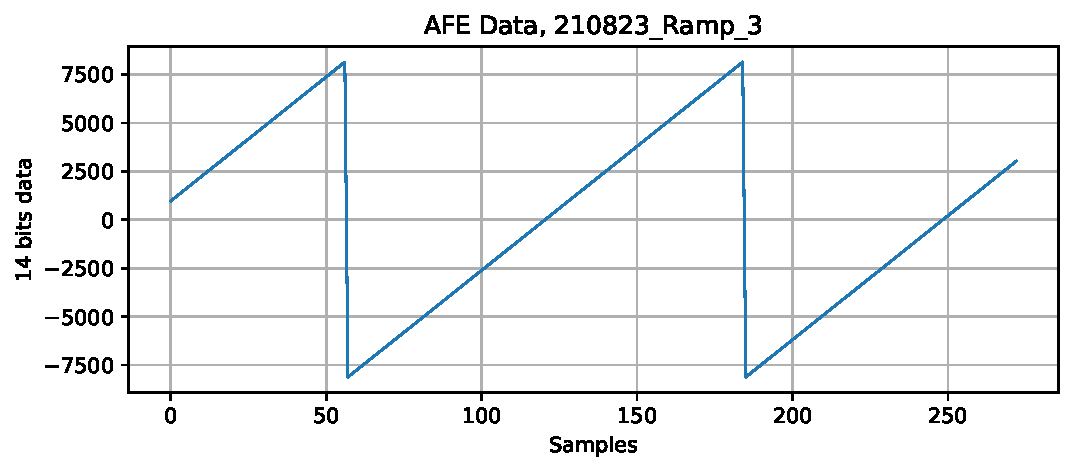
\includegraphics[width=0.9\textwidth,origin=c,angle=0]{Images/DaphneAFETest/210823_Ramp_3.pdf}
% "\includegraphics" from the "graphicx" permits to crop (trim+clip)
% and rotate (angle) and image (and much more)
\caption{\label{fig:InitPeriTask} Control and configuration task scheme.}
\end{figure}


\begin{figure}[htbp]
\centering % \begin{center}/\end{center} takes some additional vertical space
%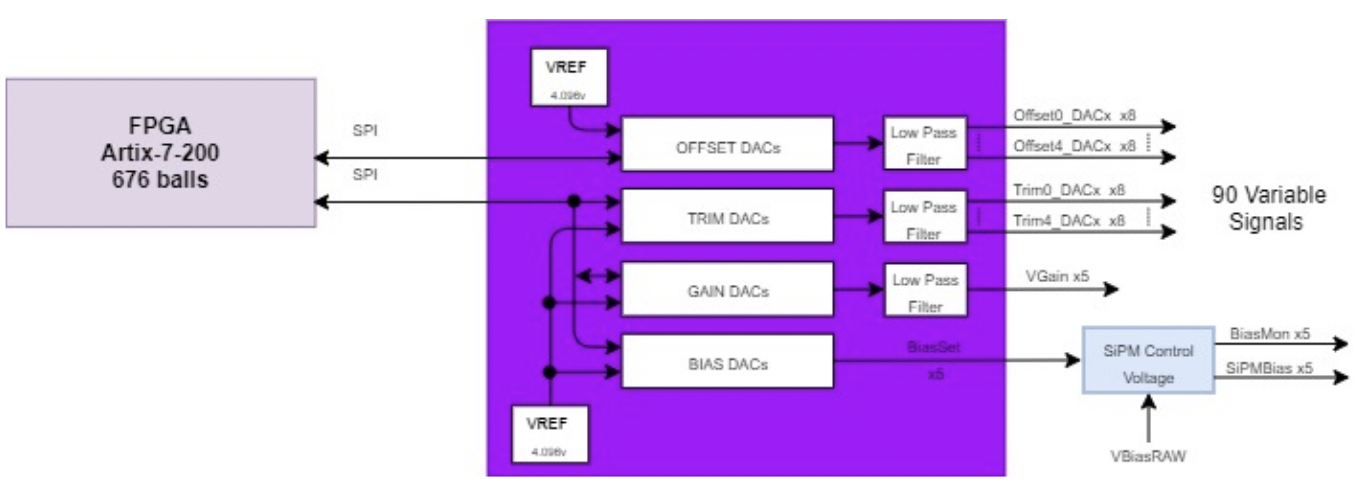
\includegraphics[width=.8\textwidth,trim=30 110 0 0,clip]{Images/BiasControl.png}
%\qquad
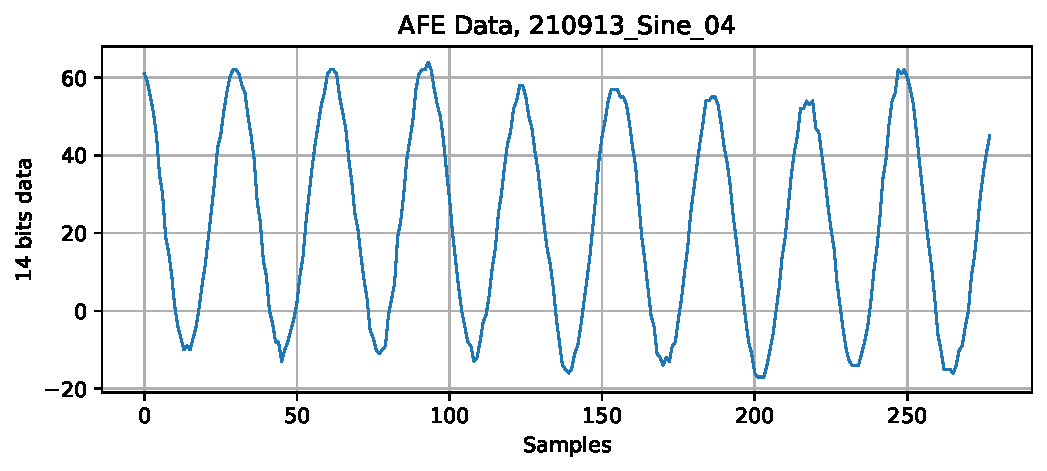
\includegraphics[width=0.9\textwidth,origin=c,angle=0]{Images/DaphneAFETest/210913_Sine_04.pdf}
% "\includegraphics" from the "graphicx" permits to crop (trim+clip)
% and rotate (angle) and image (and much more)
\caption{\label{fig:InitPeriTask} Control and configuration task scheme.}
\end{figure}


\begin{figure}[htbp]
\centering % \begin{center}/\end{center} takes some additional vertical space
%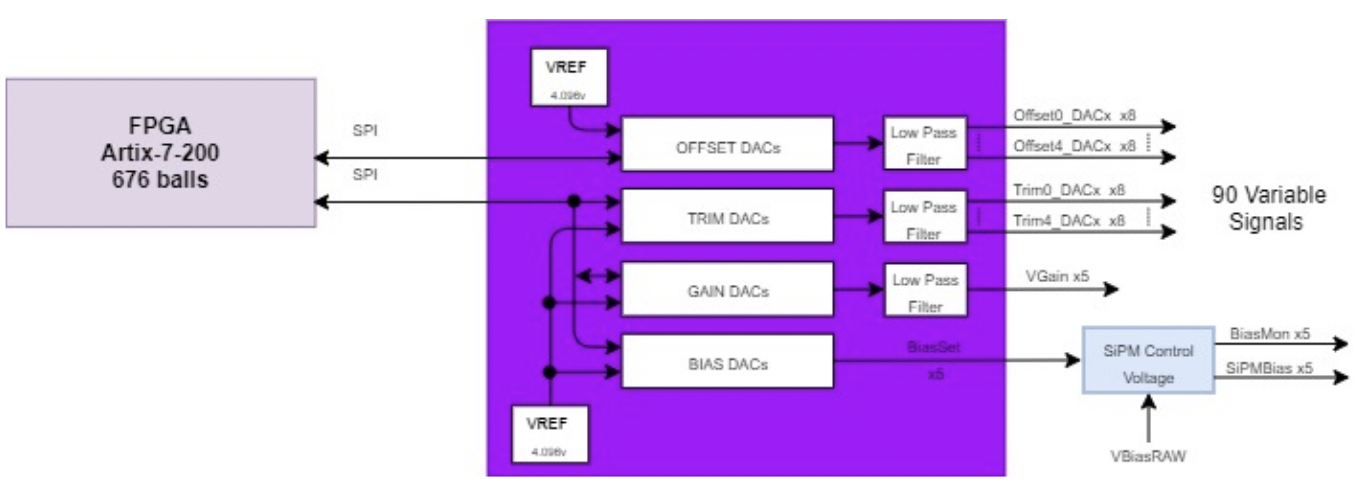
\includegraphics[width=.8\textwidth,trim=30 110 0 0,clip]{Images/BiasControl.png}
%\qquad
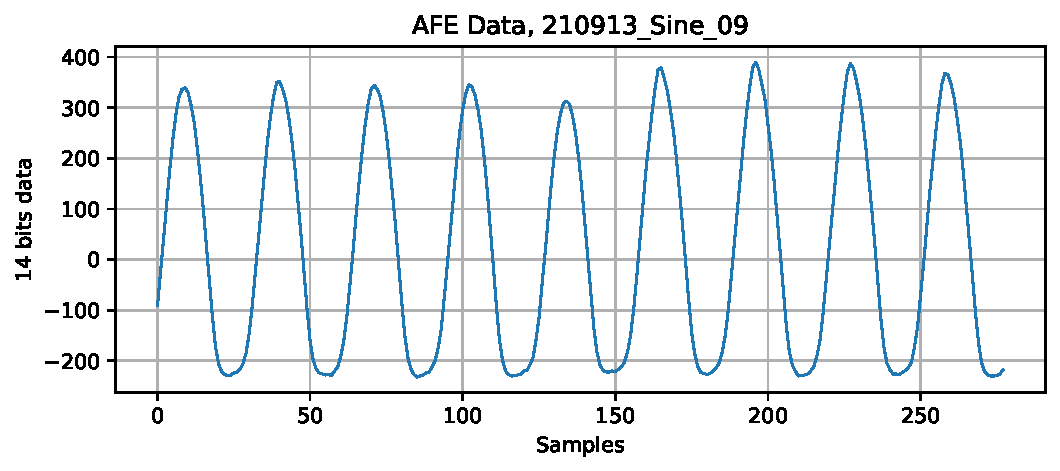
\includegraphics[width=0.9\textwidth,origin=c,angle=0]{Images/DaphneAFETest/210913_Sine_09.pdf}
% "\includegraphics" from the "graphicx" permits to crop (trim+clip)
% and rotate (angle) and image (and much more)
\caption{\label{fig:InitPeriTask} Control and configuration task scheme.}
\end{figure}



\begin{figure}[htbp]
\centering % \begin{center}/\end{center} takes some additional vertical space
%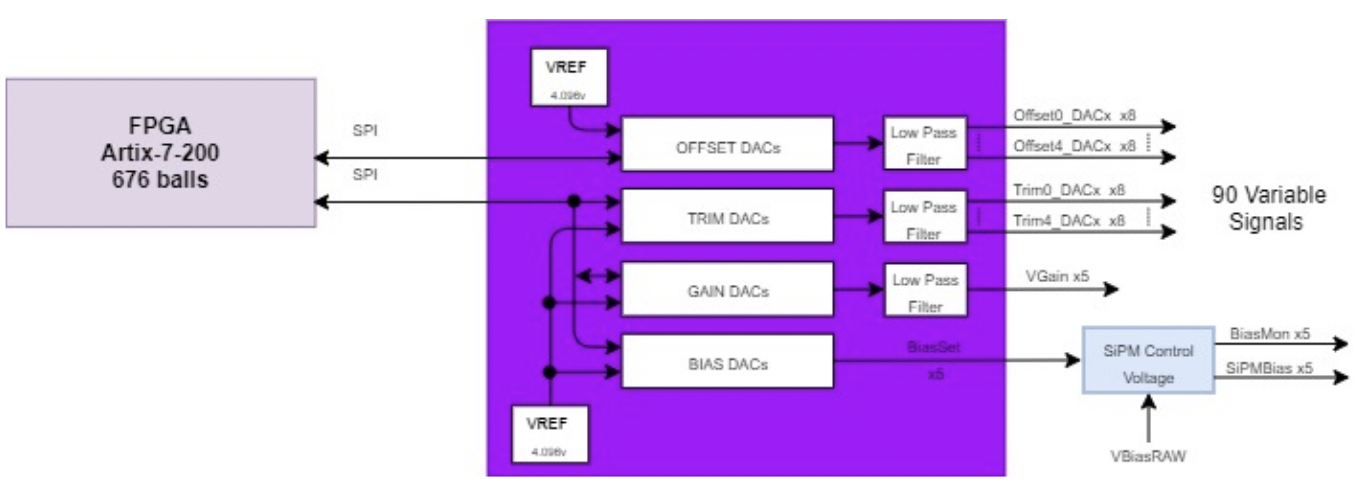
\includegraphics[width=.8\textwidth,trim=30 110 0 0,clip]{Images/BiasControl.png}
%\qquad
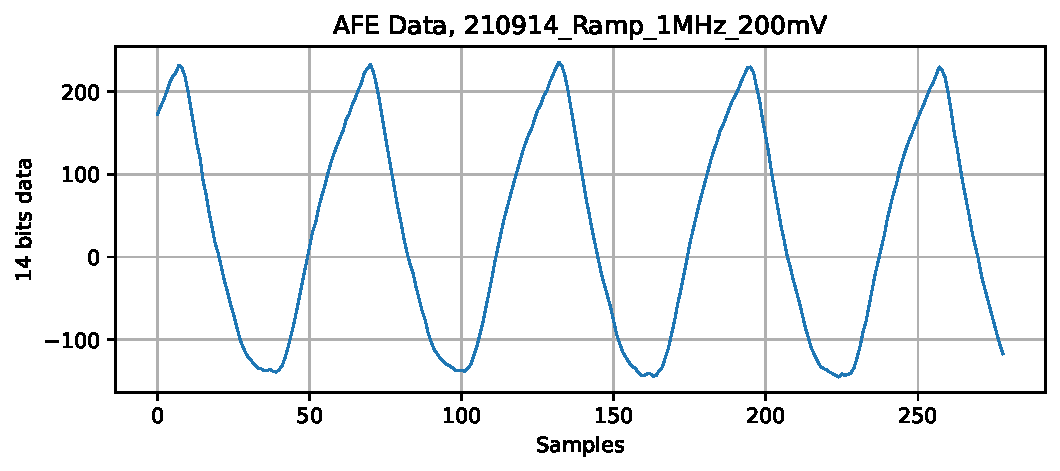
\includegraphics[width=0.9\textwidth,origin=c,angle=0]{Images/DaphneAFETest/210914_Ramp_1MHz_200mV.pdf}
% "\includegraphics" from the "graphicx" permits to crop (trim+clip)
% and rotate (angle) and image (and much more)
\caption{\label{fig:InitPeriTask} Control and configuration task scheme.}
\end{figure}

\begin{figure}[htbp]
\centering % \begin{center}/\end{center} takes some additional vertical space
%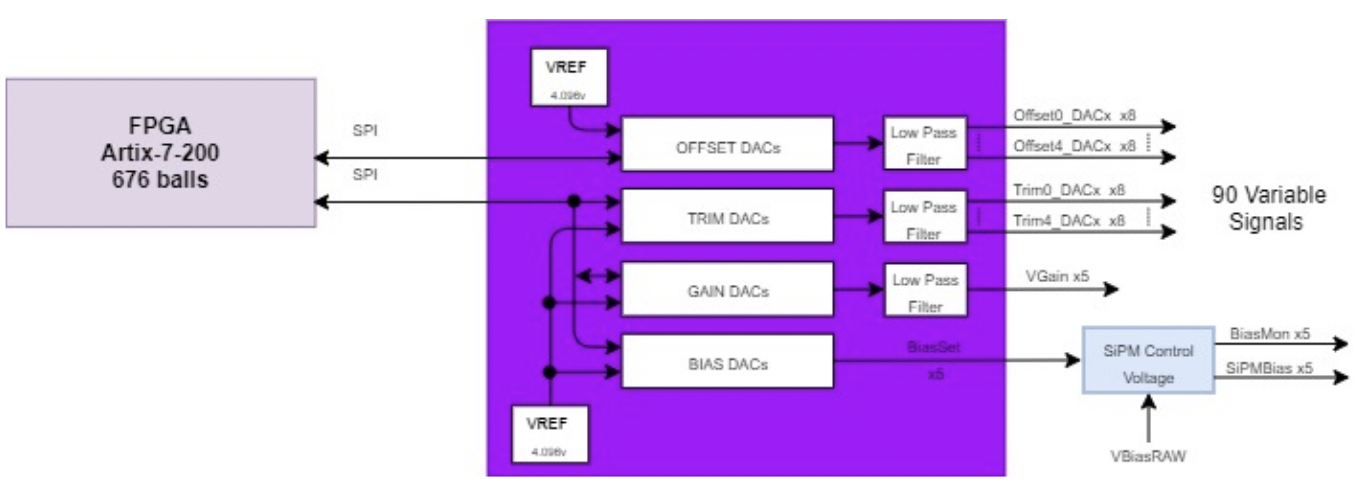
\includegraphics[width=.8\textwidth,trim=30 110 0 0,clip]{Images/BiasControl.png}
%\qquad
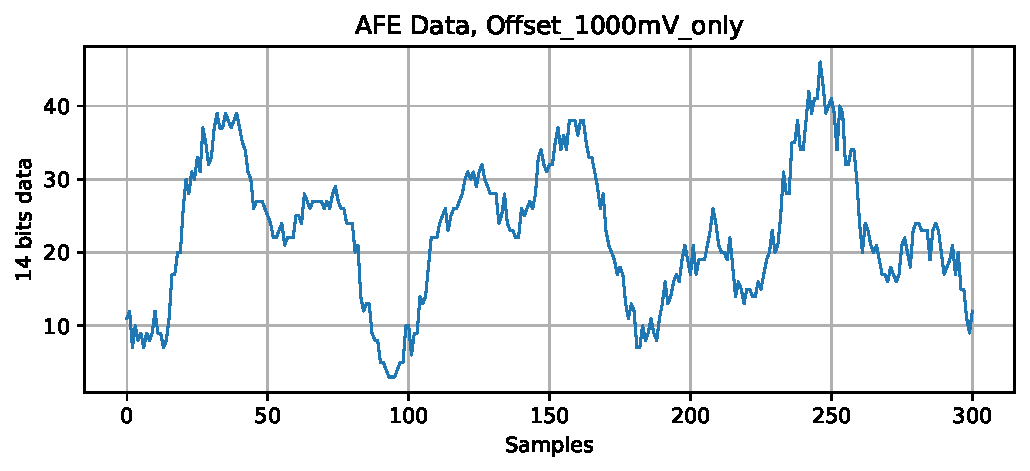
\includegraphics[width=0.9\textwidth,origin=c,angle=0]{Images/DaphneAFETest/Offset_1000mV_only.pdf}
% "\includegraphics" from the "graphicx" permits to crop (trim+clip)
% and rotate (angle) and image (and much more)
\caption{\label{fig:InitPeriTask} Control and configuration task scheme.}
\end{figure}


\begin{figure}[htbp]
\centering % \begin{center}/\end{center} takes some additional vertical space
%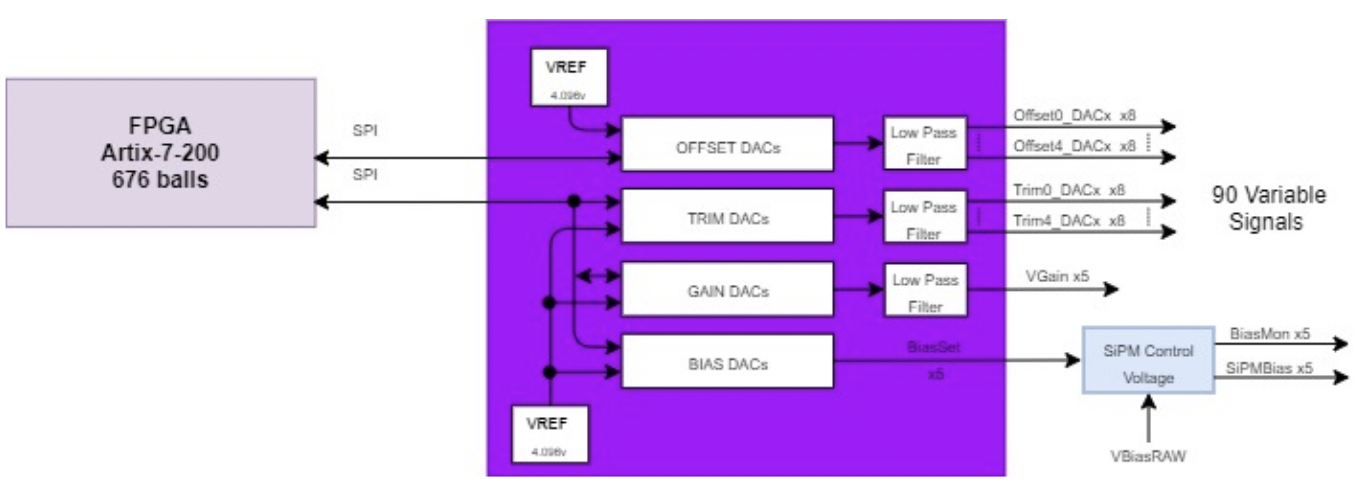
\includegraphics[width=.8\textwidth,trim=30 110 0 0,clip]{Images/BiasControl.png}
%\qquad
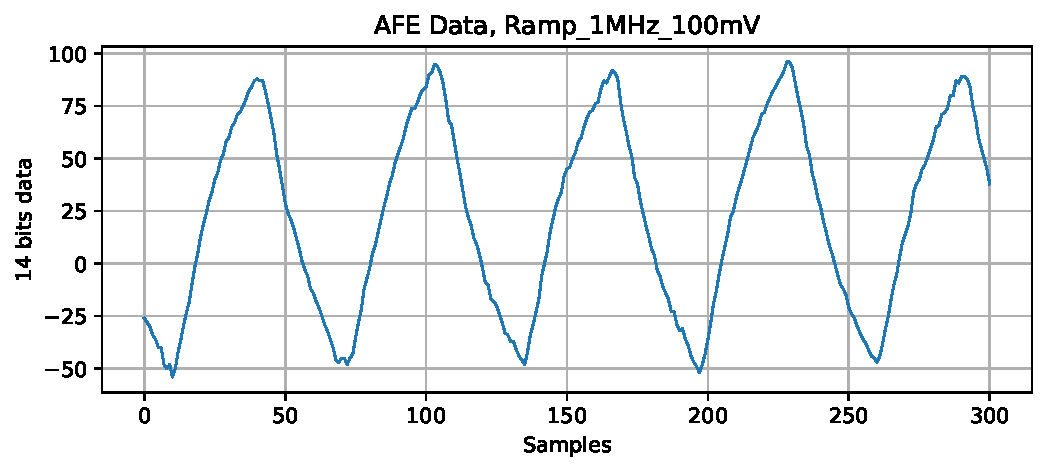
\includegraphics[width=0.9\textwidth,origin=c,angle=0]{Images/DaphneAFETest/Ramp_1MHz_100mV.pdf}
% "\includegraphics" from the "graphicx" permits to crop (trim+clip)
% and rotate (angle) and image (and much more)
\caption{\label{fig:InitPeriTask} Control and configuration task scheme.}
\end{figure}

\begin{figure}[htbp]
\centering % \begin{center}/\end{center} takes some additional vertical space
%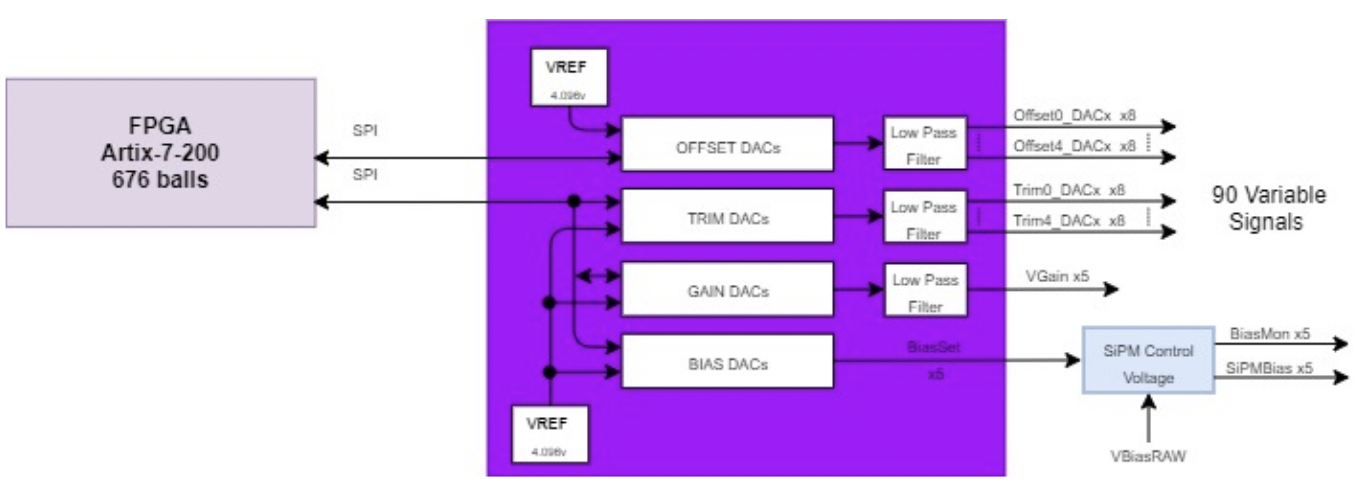
\includegraphics[width=.8\textwidth,trim=30 110 0 0,clip]{Images/BiasControl.png}
%\qquad
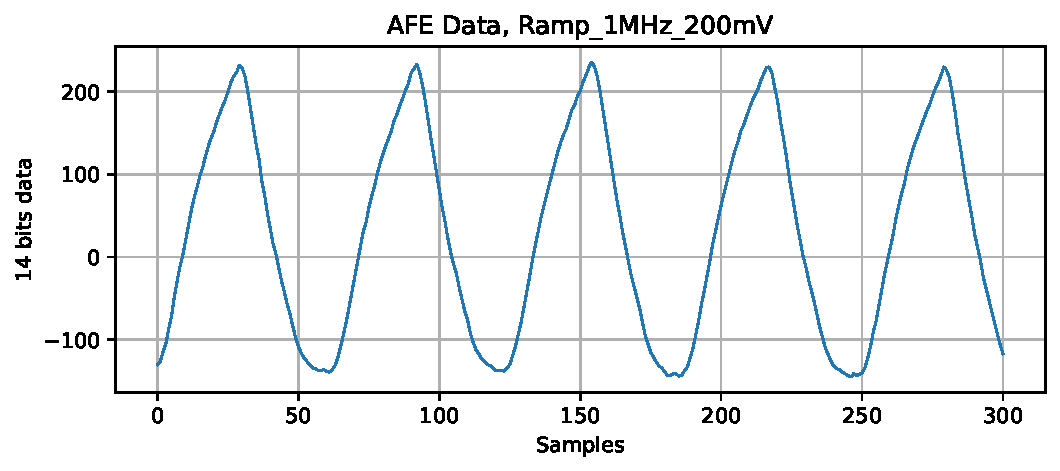
\includegraphics[width=0.9\textwidth,origin=c,angle=0]{Images/DaphneAFETest/Ramp_1MHz_200mV.pdf}
% "\includegraphics" from the "graphicx" permits to crop (trim+clip)
% and rotate (angle) and image (and much more)
\caption{\label{fig:InitPeriTask} Control and configuration task scheme.}
\end{figure} 
        

        

        

\section{DAPHNE test results}
\subsection{DAPHNE: cold and warm electronics interface}

The DAPHNE board is the warm electronics interface with the cold electronics that will operate outside the criostat. DAPHNE provides power to both amplifier and SiPMs, re-amplifies and digitizes the signals from the PD modules, formats and transmits the generated data to the DAQ system of the experiment. 

\begin{figure}[h]
\centering
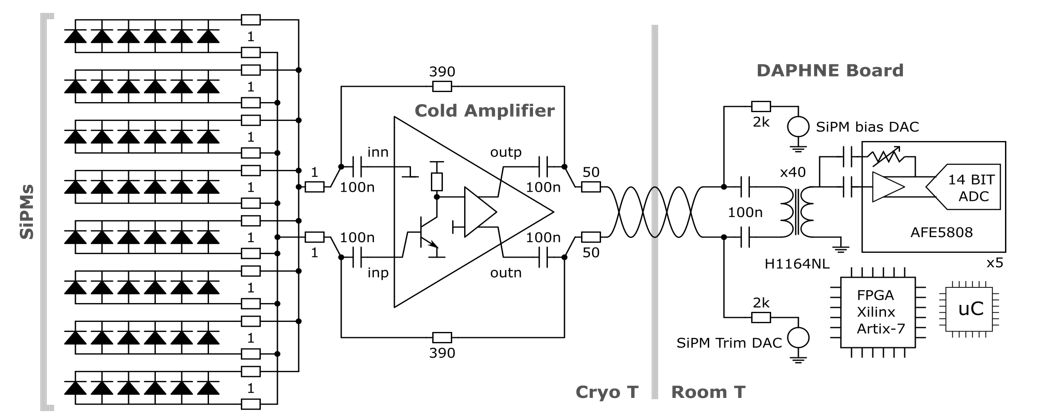
\includegraphics[width=100mm]{Images/pd_electronics.png}
\caption[]{Schematic of the PD cold and warm electronics.}
\label{fig:pd_electronics}
\end{figure}

At Milano-Bicocca, our main focus with the DAPHNE development is the interface between DAPHNE's analog front end (AFE), the Texas Intruments AFE5808 and the cold electronics, to achieve the best possible signal fidelity, SNR, demonstrate the capability to trigger on single P.E. signal and to control precisely the trigger level in each channel.

In the following subsections, various test that were instrumental to advance towards the demostration that the PD electronics system can comply with the DUNE's experiment requirements. 

\subsection{Dynamic range and signal fidelity}

The dynamic range requirement for the PD system is 2000 photoelectrons. According to the simulation and measured data, a single P.E. can be considered to have a peak to peak value of around 400 ${\mu}V$ for 45\% PDE at the input of DAPHNE's AFE. The AFE5808 \cite{afe5808a} can safely be configured to have a linear response for an input signal up to $1Vpp$. Considering that 2000 P.E. is around 800 $mVpp$, the AFE5808 should handle the required dynamic range with a 20\% safety margin. There is although a drawback, the AFE5808 has no configurable OFFSET for the first stage low-noise amplifier (LNA) reference voltage and since the SiPMs signals are in escence unipolar signals, only half of the dynamic range can be exploited. To address this issue, DAPHNE designers had to implement an external OFFSET correction circuit to modify the reference voltage at the input of the LNA to allow the full dynamic range to be exploited.

\begin{figure}[h]
\centering
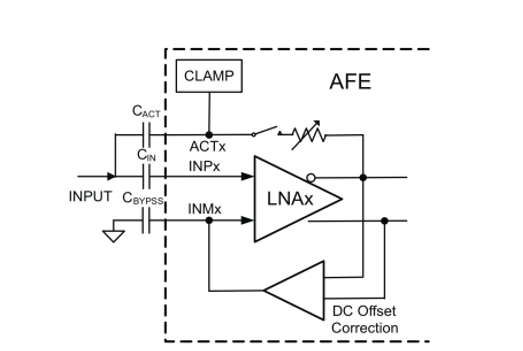
\includegraphics[width=100mm]{Images/AFE5808_frontend.png}
\caption[]{Schematic the AFE5808 input LNA, active termination and DC offset correction. \cite{afe5808a}}
\label{fig:afe_frontend}
\end{figure}

Figure \ref{fig:afe_frontend} shows the input LNA. The signal arrives from the cold amplifier via twisted pair and passes throught a 1:1 balun transformer to perform the differential to single ended convertion and finally gets terminated by the AFE5808's active termination circuit $ACTx$. The active termination is user configurable, but in order to match the system impedance, 100$\Omega$ termination must be selected. The OFFSET correction circuit is not shown but is simple in nature, it consist in a DAC (Digital to Analog Converter) connected to the $INPx$ pin via a 20 $k\Omega$ resistor, making a voltage divider with the internal pull-up resistor and voltage reference.

\begin{figure}[h]
\centering
\subfigure[]{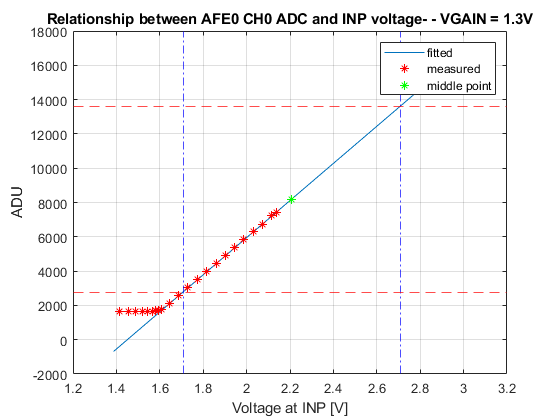
\includegraphics[width=60mm]{Images/linear_vgain_13.png}}
\subfigure[]{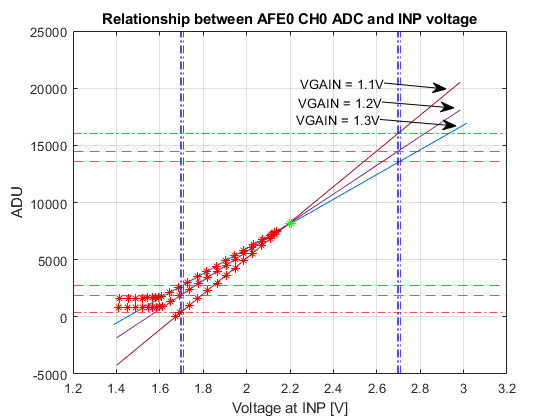
\includegraphics[width=60mm]{Images/linear_vgain_all.png}}
\caption[]{Linearity response of the AFE5808 and the OFFSET circuit. a) Attenuation: VGAIN 1.3V. b) Attenuation: VGAIN 1.1V - 1.2V - 1.3V.  }
\label{fig:offset_test}
\end{figure}

Figure \ref{fig:offset_test} shows the response of the AFE5808 when the OFFSET circuit is set to a specific value. Both figures \ref{fig:offset_test}a and \ref{fig:offset_test}b show the relatioship between the measured voltage at $INPx$ and the average $ADU$ (Analog Digital Unit) acquired by DAPHNE in channel 0. The vertical blue lines indicate the limits of the linear input of $1Vpp$, and the horizontal red lines are the intersection of the blue lines with the fitted line of the measured data, which indicate the expected linear region in $ADU$ units. The green asterisk indicate the midpoint OFFSET where the maximun voltage swing can be obtained for a sinusoidal voltage input. Note that for high attenuation configurations, the AFE5808 clamp effect can be noted at low ADU values but there is still a small linear region below $1Vpp$ (horizontal red lines) guaranteed linear zone. The effect of decreasing the attenuation can be seen in figure \ref{fig:offset_test}b, where the AFE5808 can be configured to have full linear range for $2^{14}$ ADU, as is for the case of $VGAIN = 1.1V$ (VGAIN is the programmable attenuator voltage control) where the clamping effect is below and above the ADU range giving a straight line for every voltage range at $INP$. This relationship estimates the overall gain of each AFE5808 channel at specific configuration, and has units of $\frac{ADU}{V}$. 

The signal fidelity of the acquired waveforms was a concern, specially the effect of the OFFSET correction circuit could have in the internal amplification and digitization processes of the AFE5808. A sinusoidal signal with a 200 $mVpp$ is injected at the input and waveforms are acquired stepping OFFSET values. Figure \ref{fig:fidelity_1} shows the acquired sinusoidal waveform at the top. The bottom waveforms were acquired with an oscilloscope probing the $INP$ node of the AFE5808 channel that is under test. As can bee seen in figure \ref{fig:fidelity_1}a, both waveforms present a clipping effect that distorts the signal. According to what was presented above, this clipping effect should not occur at this point and moreover, it's occurring at the opposite semicycle as the ADU OFFSET moves towards 0. 

\begin{figure}[h]
\centering
\subfigure[]{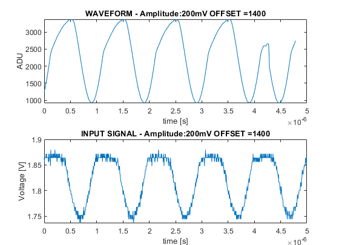
\includegraphics[width=60mm]{Images/fidelity_200.png}}
\subfigure[]{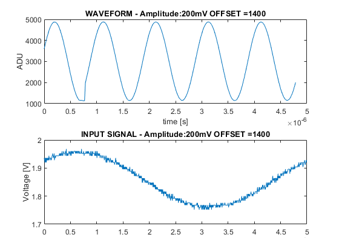
\includegraphics[width=60mm]{Images/fidelity_200_corrected.png}}
\caption[]{Acquired waveforms when a sinusoidal signal is injected at the input of the AFE5808. a) 100 $\Omega$ active termination ON . b) Active termination OFF (passive $100 \Omega$ termination) }
\label{fig:fidelity_1}
\end{figure}

It was noted that the active termination circuit $ACTx$, shown in figure \ref{fig:afe_frontend}, has a clamp feature. After deliberation, it was concluded that the clipping issue may have the following explanation: As the $INP$ value decreases due to the effect of the OFFSET correction, the inverted DC output value of the LNA increases moving closer to the CLAMP activation value. The CLAMP can be removed by deactivating the $ACTx$ circuit, breaking the feedback loop. At this point, a physical $100\Omega$ resistor had to be added in order to correctly terminate the line. Figure \ref{fig:fidelity_1}b shows the result of these modifications, where both acquired and probed signals no longer suffer from the clipping effect. 

\begin{figure}[h]
\centering
\subfigure[]{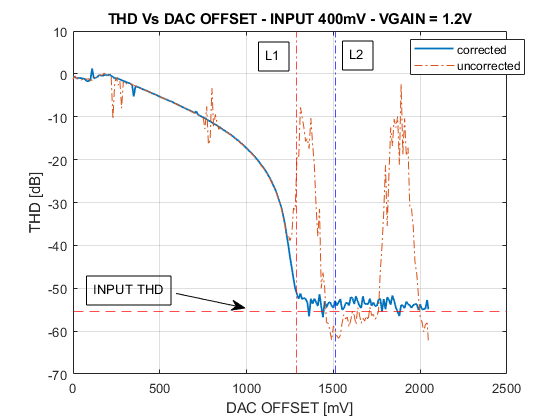
\includegraphics[width=60mm]{Images/thd_1.png}}
\subfigure[]{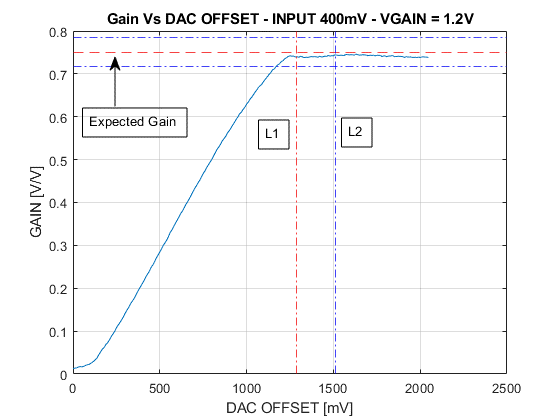
\includegraphics[width=60mm]{Images/gain_1.png}}
\caption[]{Total harmonic distortion (THD) and GAIN of the acquired signal for stepping values of OFFSET configuration.  a) THD b) GAIN }
\label{fig:thd_gain}
\end{figure}

Having solved the aforementioned issue and in order to quantify the fidelity of the acquisition with respect of the OFFSET configuration, measurements of the total harmonic distortion and signal gain were performed with stepping OFFSET configurations. Figure \ref{fig:thd_gain}a shows the THD figures for different OFFSET configurations. A $400 mVpp$ sinusoidal signal was injected and probed at the input. The input THD from the probed signal was calculated and serves as a reference (red dashed line) for the THD calculations of the acquired waveforms. The figure can be explained as follows: As the OFFSET value increases towards the midpoint, the THD figures should improve towards the limit of the reference THD value. The limit at which the acquired THD reaches the reference can be estimated using the data from figure \ref{fig:offset_test}b, denoted $L1$ and $L2$, marks the beginning of the OFFSET linear regions. Figure \ref{fig:thd_gain}b shows the gain for stepping OFFSET values where the expected gain can also be estimated from the referred data in figure \ref{fig:offset_test}b. For both figures \ref{fig:thd_gain}a and \ref{fig:thd_gain}b, the measured THD and gain values approximates to the expected values in the expected linear region, therefore, it is concluded that the OFFSET correction circuit does not have a degrading effect in the signal fidelity of the acquired waveforms.  

\subsection{Noise issues in the DAPHNE board}

In the previous subsection, an effort has been made to achieve the best possible signal fidelity and to guarantee that the subsystems around the AFE do not affect the acquisition mechanisms. Large test signals were injected to verify the fidelity and a serious problem was identified and resolved. Moving forward to small signals, in the range of single P.E. waveforms, the main concern is to achieve the lowest noise figures possible to obtain the best SNR. 

The first calibrations tests integrating the cold amplifier with DAPHNE failed. Even at large amplification factors, DAPHNE had very poor SNR performance.  

Figure \ref{fig:noise_1} shows the average frequency spectrum of 10000 waveforms. The yellow plot shows various spurious frequency components peaks, from these, two peaks show larger amplitude, 630 $kHz$ and 1.53 $MHz$. At this point, the DAPHNE board was probed extensively to search and pinpoint the origin of these components. The noise components was found to be injected at the input nodes before the capacitors that decouple the bias and trim circuitry to power the SiPMs, and originate from the DC-DC voltage converters circuitry, where the 48V input voltage gets converted to the numerous voltage rails that DAPHNE subsystems power from, specifically the +5V, -5V analog and SiPM bias voltage rails.

The referred noise from the power rails affected subsystems that were directly connected to the AFEs input and are critical for the PD systems performance and monitoring. These systems are:

\begin{enumerate}
    \item The analog multiplexer for the SiPMs current monitor systems
    \item The BIAS supply circuitry.
    \item the BIAS TRIM voltage circuitry. 
\end{enumerate}

The cited subsystems were found to be vulnerable due to inadequate PSSR (Power Supply Rejection Ratio). Figure \ref{fig:noise_1} also shows spectrum figures when these subsystems are disconnected, confirming that the overall noise gets injected through them via their power supply rails. 

\begin{figure}[h]
\centering
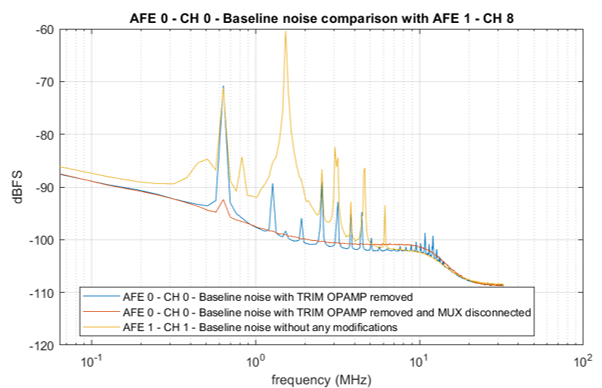
\includegraphics[width=100mm]{Images/noise_1.png}
\caption[]{Average frequency spectrum of acquire signals.}
\label{fig:noise_1}
\end{figure}

The approach taken to solve this problem was to apply filter patches at the output of these subsystems given that it was not possible to apply filters at the source of the noise, the DC-DC converters, without the risk of seriously damaging the boards in the process. Three different patches were applied and each of them with satisfactory results. 

The patch was selected considering the number of extra components and difficulty of implementation. Figure \ref{fig:patches}a show the schematic of the selected filter patch, where an extra capacitor and resistor were inserted after the TRIM node to form a low pass filter. Also, an extra capacitor was inserted between GND and S2 was inserted to filter noise components that are injected through this node. The other patches 1 and 2 are not shown, but they produce the same result with slight variations of patch 3. Other changes that were made are the addition of inductors at the subsystem's power rails to increase the PSSR, and changes to components in the BIAS circuitry to filter better the SiPMs BIAS voltages. Figure \ref{fig:patches}b show the frequency spectrum of the input after the patches are applied to different AFE chips. The overall comparison show similar noise suppression results for each patch applied. There is still one noise component that could not be suppressed, which is believed to be injected via the power rails of the AFE chip itself, where it is not possible to insert a filter without seriously risking the integrity of the board. 

\begin{figure}[h]
\centering
\subfigure[]{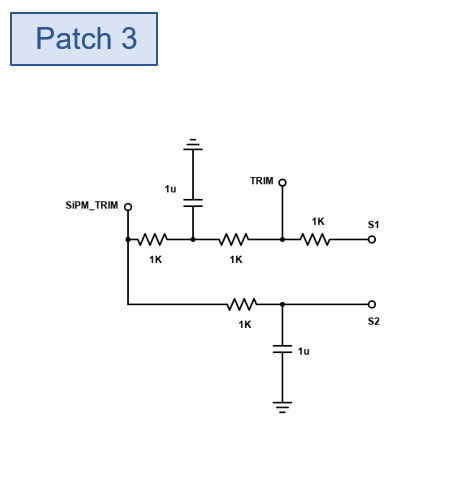
\includegraphics[width=60mm]{Images/patch_3.png}}
\subfigure[]{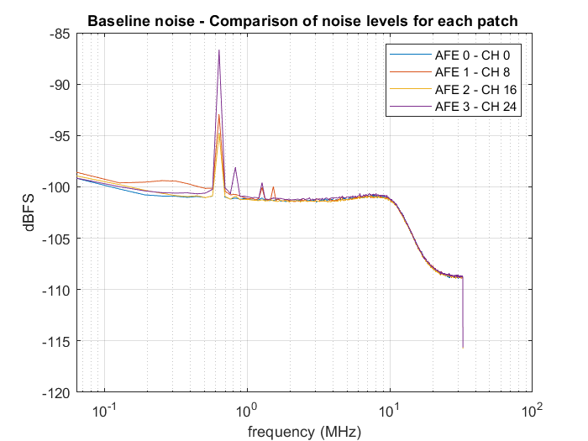
\includegraphics[width=60mm]{Images/noise_comp_patch.png}}
\caption[]{Selected filter patch at the Analog Multiplexer and TRIMM output.  a) S1 ans S2 are the analog multiplexer pins. TRIM is the BIAS TRIM voltage output. b)  Frequency spectrum  of the AFE input after the patches were applied.}
\label{fig:patches}
\end{figure}


\subsection{Cold amplifier: SNR and P.E. dynamic range}

Previous sections show test and studies performed to obtain the best SNR and dynamic range possible for DAPHNE's AFE systems. These tests were key to identify issues for both performance figures and apply modifications to the hardware in order to improve performance as was showed.

With the issues addressed, integration test of the cold and warm electronics (DAPHNE) were performed. The firsts tests were done with a very high AFE gain configuration to have a starting point to tune the systems to achieve the goals of a SNR greater than 4 and a dynamic range of 2000 P.E. The AFE gain configuration that was used for the following test was a LNA gain of $12dB$, a programmable gain amplifier PGA gain of $24dB$ and the PGA and LNA integrators ON. The cold amplifier ganging 48 SiPMs were submerged in $LN_2$, introduced into a dark box where a LED driver pulses light into the detectors via a optical fiber. The LED driver triggers with a external signal synchronized to the external trigger signal for DAPHNE.

Figure \ref{fig:fbk_hist_avg_vgain_03} show the results of the tests. The histogram in figure \ref{fig:fbk_hist_avg_vgain_03}a is produce by the integration of 40 samples after the beginning of the rising edge of the average signal. Figure \ref{fig:fbk_hist_avg_vgain_03}b shows the average single P.E. signal produced by averaging every waveform whose integral matches the second peak of the histogram. By taking the first and second peaks of the histogram, corresponding to noise and single P.E. charge respectively, the SNR figure used on-wards is defined as:

\begin{equation}
    SNR = \frac{\Delta}{\sigma_0}
\label{eq:SNR}
\end{equation}

where delta is defined as $\Delta = \mu_1 - \mu_0$ the distance between the mean values of the Gaussian fits of the peaks, shown in red, and $\sigma_0$ is the standard deviation of the fit of the peak corresponding to noise integral, the first peak. The dynamic range is defined as the peak-to-peak value of the average P.E. over the full range of the AFE ADC, in this case, $2^{14}$. 

\begin{equation}
    DR = \frac{A_{pp}}{2^{14}}
\label{eq:DR}
\end{equation}

\begin{figure}[h]
\centering
\subfigure[]{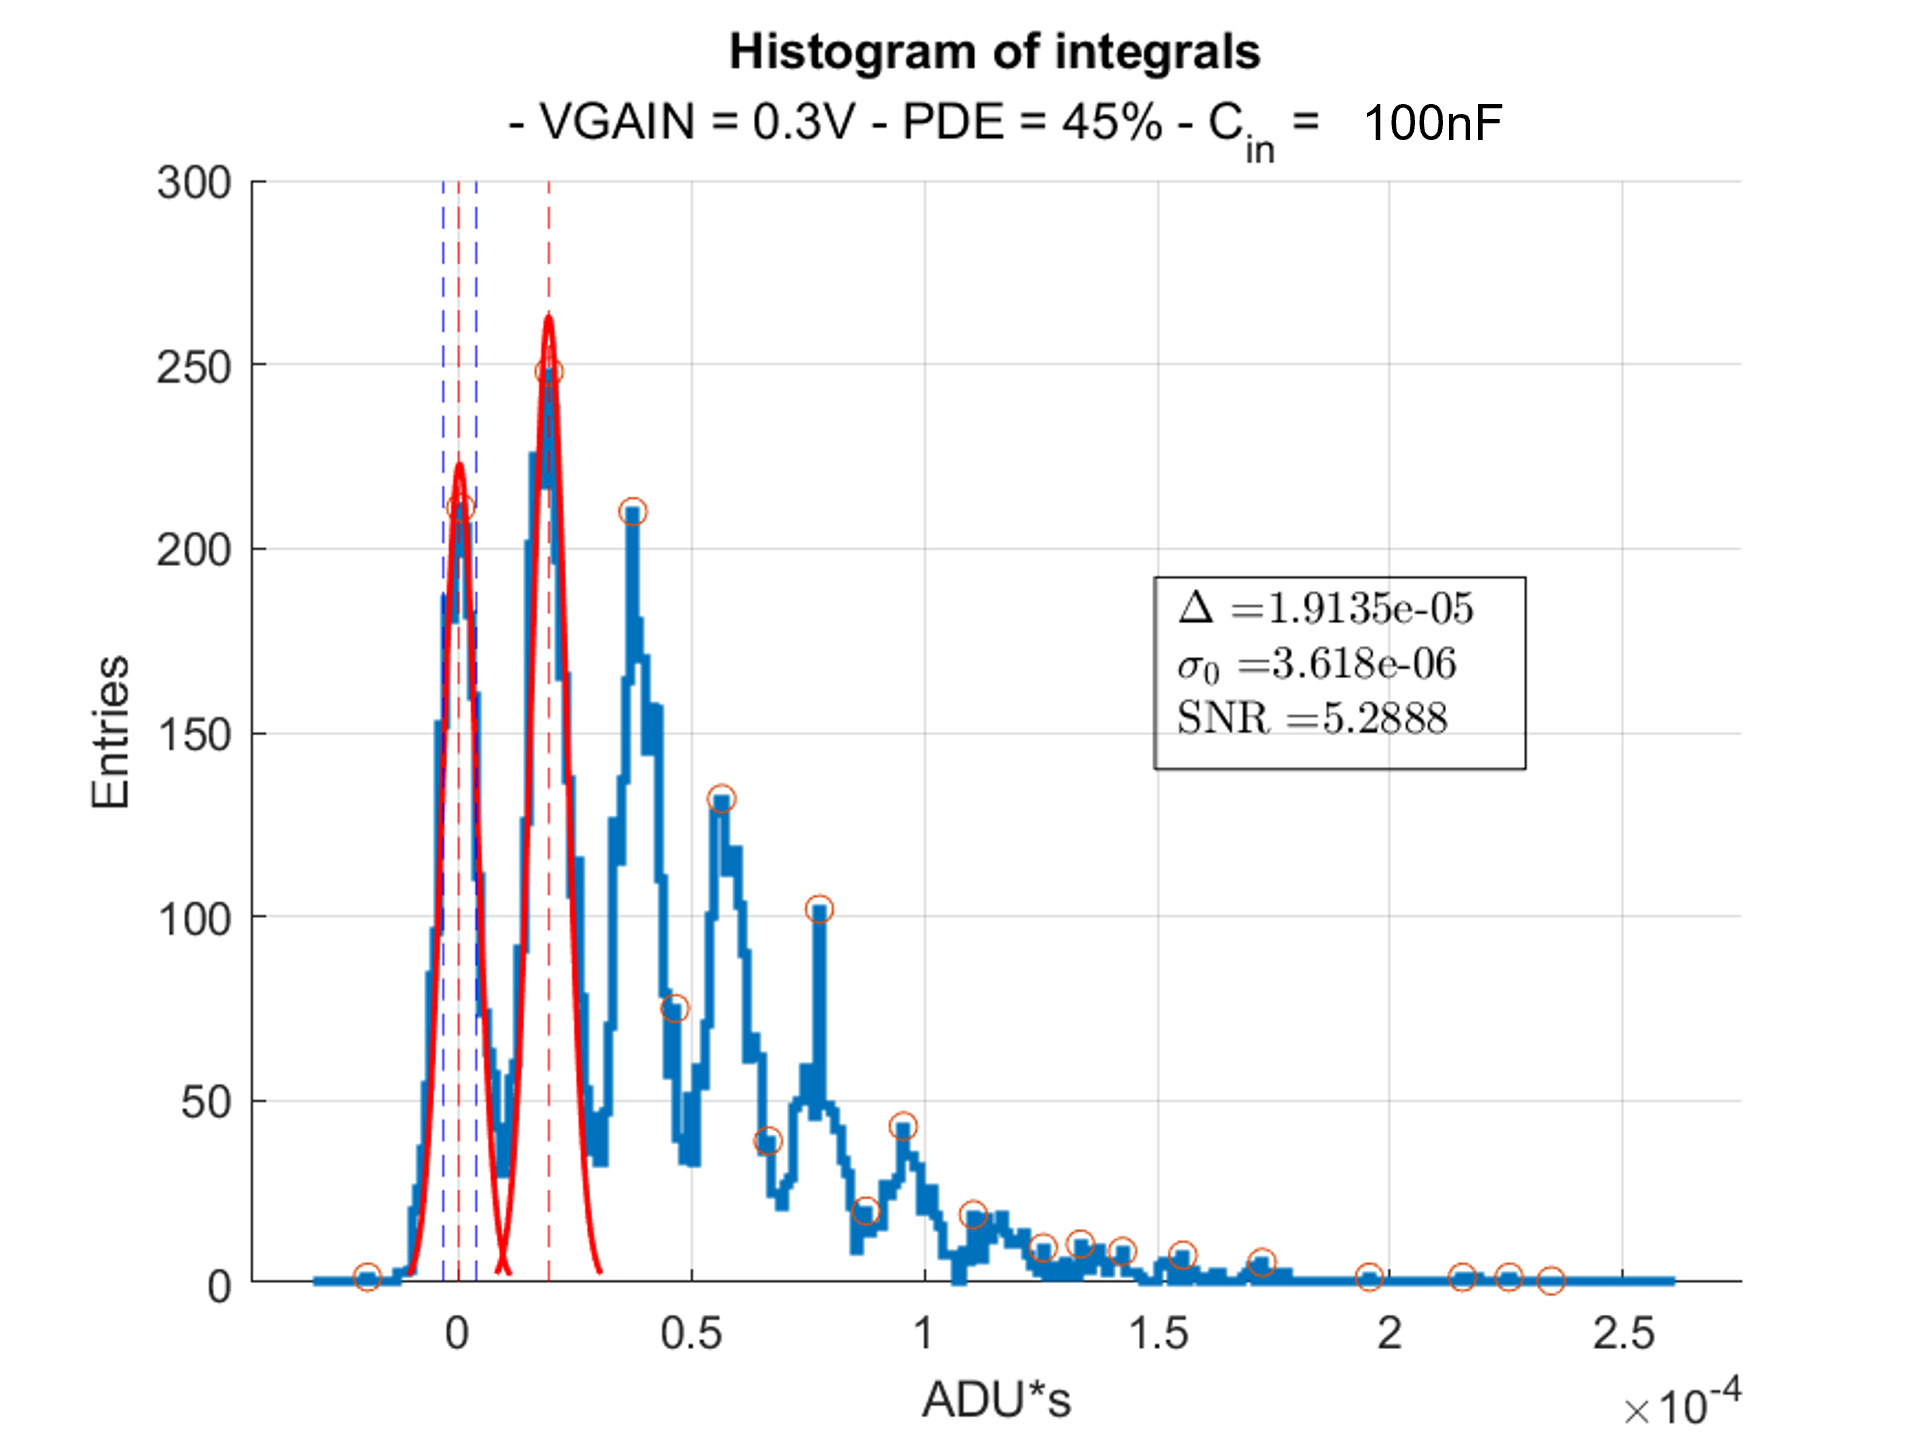
\includegraphics[width=60mm]{Images/hist_fbk_vgain_03.png}}
\subfigure[]{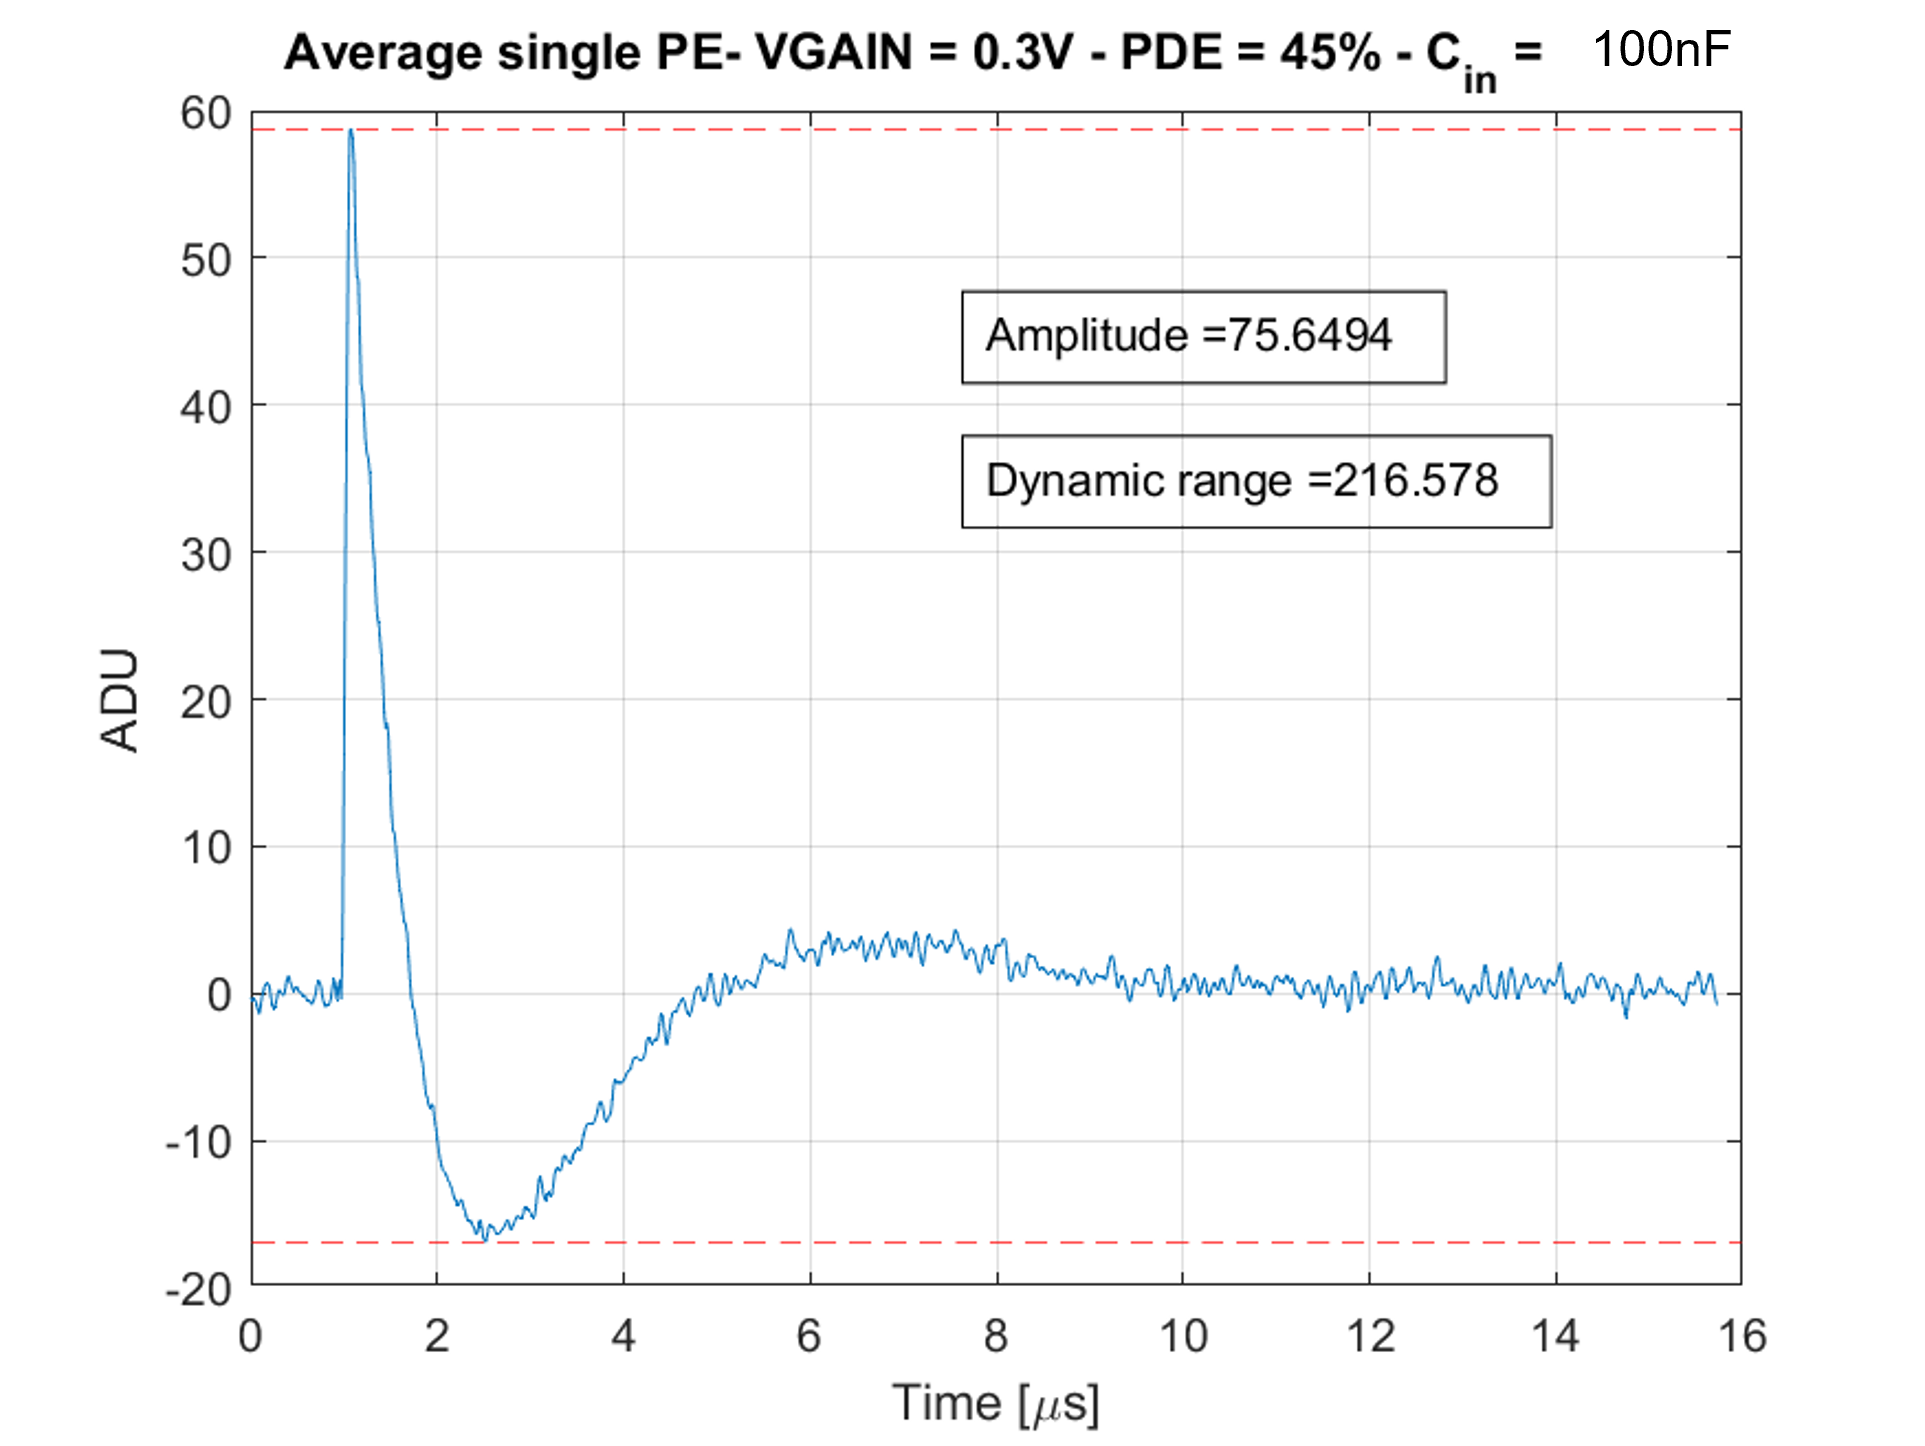
\includegraphics[width=60mm]{Images/avg_fbk_vgain_03.png}}
\caption[]{FBK-3T SiPMs cold-warm electronics integration test with VGAIN = 0.3V.  a) Histogram of charge integrals. b) Average single P.E.}
\label{fig:fbk_hist_avg_vgain_03}
\end{figure}

Applying equations \ref{eq:SNR} and \ref{eq:DR} to the data in figure \ref{fig:fbk_hist_avg_vgain_03}, a SNR of $5.29$ and a DR of $216$ P.E. is obtained. Although the SNR values comply with the requirement, the dynamic range is well below the 2000 P.E. mark. In order to calibrate the system, the following procedure was performed:

\begin{enumerate}
    \item For a given PDE configuration, in this case 45\%, and given VGAIN = 0.3V which has an overall gain of 23.4 according to the AFE5808 datasheet, the average single P.E. peak-to-peak amplitude is found by: \begin{equation}
        A_{1P.E.(0.3V)} = \frac{2^{14}}{216} = 76 ADU
    \end{equation}
    \item The target amplitude for 2000 P.E. is:
    \begin{equation}
        A_{2000P.E.} = \frac{2^{14}}{216} = 8 ADU
    \end{equation}
    \item The desired gain to obtain a single P.E. of amplitude 8 ADU is 
    \begin{equation}
        G_{1P.E.(8ADU)} = \frac{A_{2000P.E.}G_{0.3V}}{A_{1P.E.(0.3V)}} = \frac{8*23.4}{76} = 2.46(7.83)
    \end{equation}
\end{enumerate}

Taking as a reference table 16 of the AFE5808 datasheet \cite{afe5808a}, which give the overall gains values at 0.1V VGAIN intervals, a fit was performed to obtain the VGAIN value to have a gain of $7.83dB$, resulting in a VGAIN configuration of 0.86V, which gives a DR = 1919 P.E. Increasing VGAIN to $0.89V$, a DR = 2177 P.E. with a SNR = 4.34 was obtained, as can be seen in figure \ref{fig:fbk_hist_avg_vgain_2000}.

\begin{figure}[h]
\centering
\subfigure[]{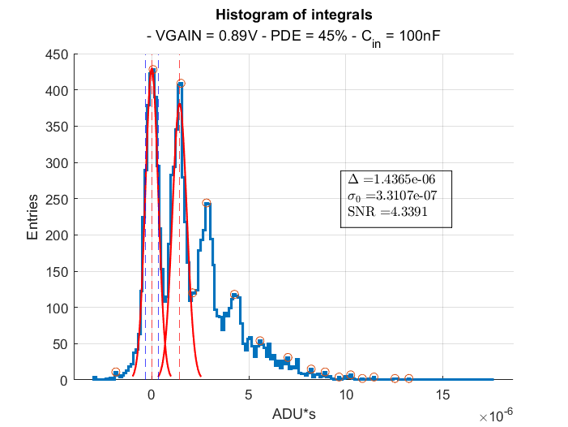
\includegraphics[width=60mm]{Images/hist_fbk_vgain_2000.png}}
\subfigure[]{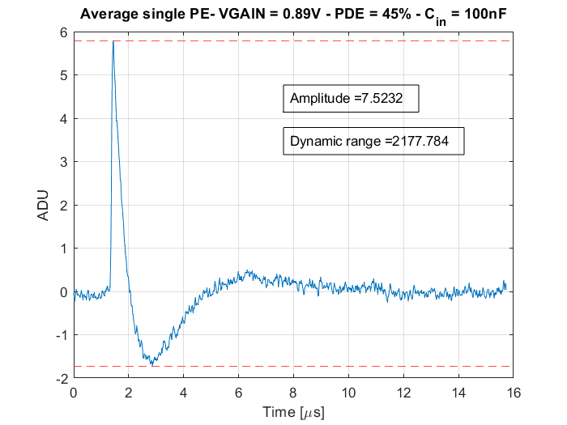
\includegraphics[width=60mm]{Images/avg_fbk_vgain_2000.png}}
\caption[]{FBK-3T SiPMs cold-warm electronics integration test with VGAIN = 0.89V.  a) Histogram of charge integrals. b) Average single P.E.}
\label{fig:fbk_hist_avg_vgain_2000}
\end{figure}

Until now, all test were performed with the AFE integrators ON. The AFE integrators are internal DC compensation that have the behavior of a high pass filter with a cut-off frequency of 80kHz. Given that the integrators act as a high pass filter, the waveforms are always centered at mid-range scale reducing the dynamic range in half and therefore, they must be disabled.

Figure \ref{fig:fbk_noise_1f}b shows a notable deterioration of the SNR figures when the LNA and PGA integrators are OFF. This main cause for this deterioration is the presence of a $1/f$ spectrum component seen in figure \ref{fig:fbk_noise_1f}a which does not allow a stable pedestal value. Also, there is the fact that the integration process is susceptible to low frequency components. 

\begin{figure}[h]
\centering
\subfigure[]{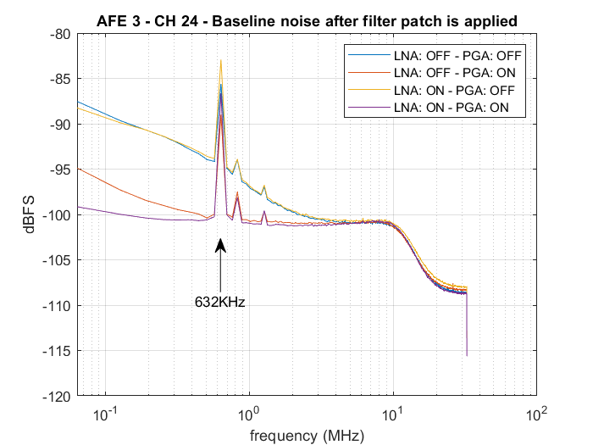
\includegraphics[width=60mm]{Images/noise_int_off_1f.png}}
\subfigure[]{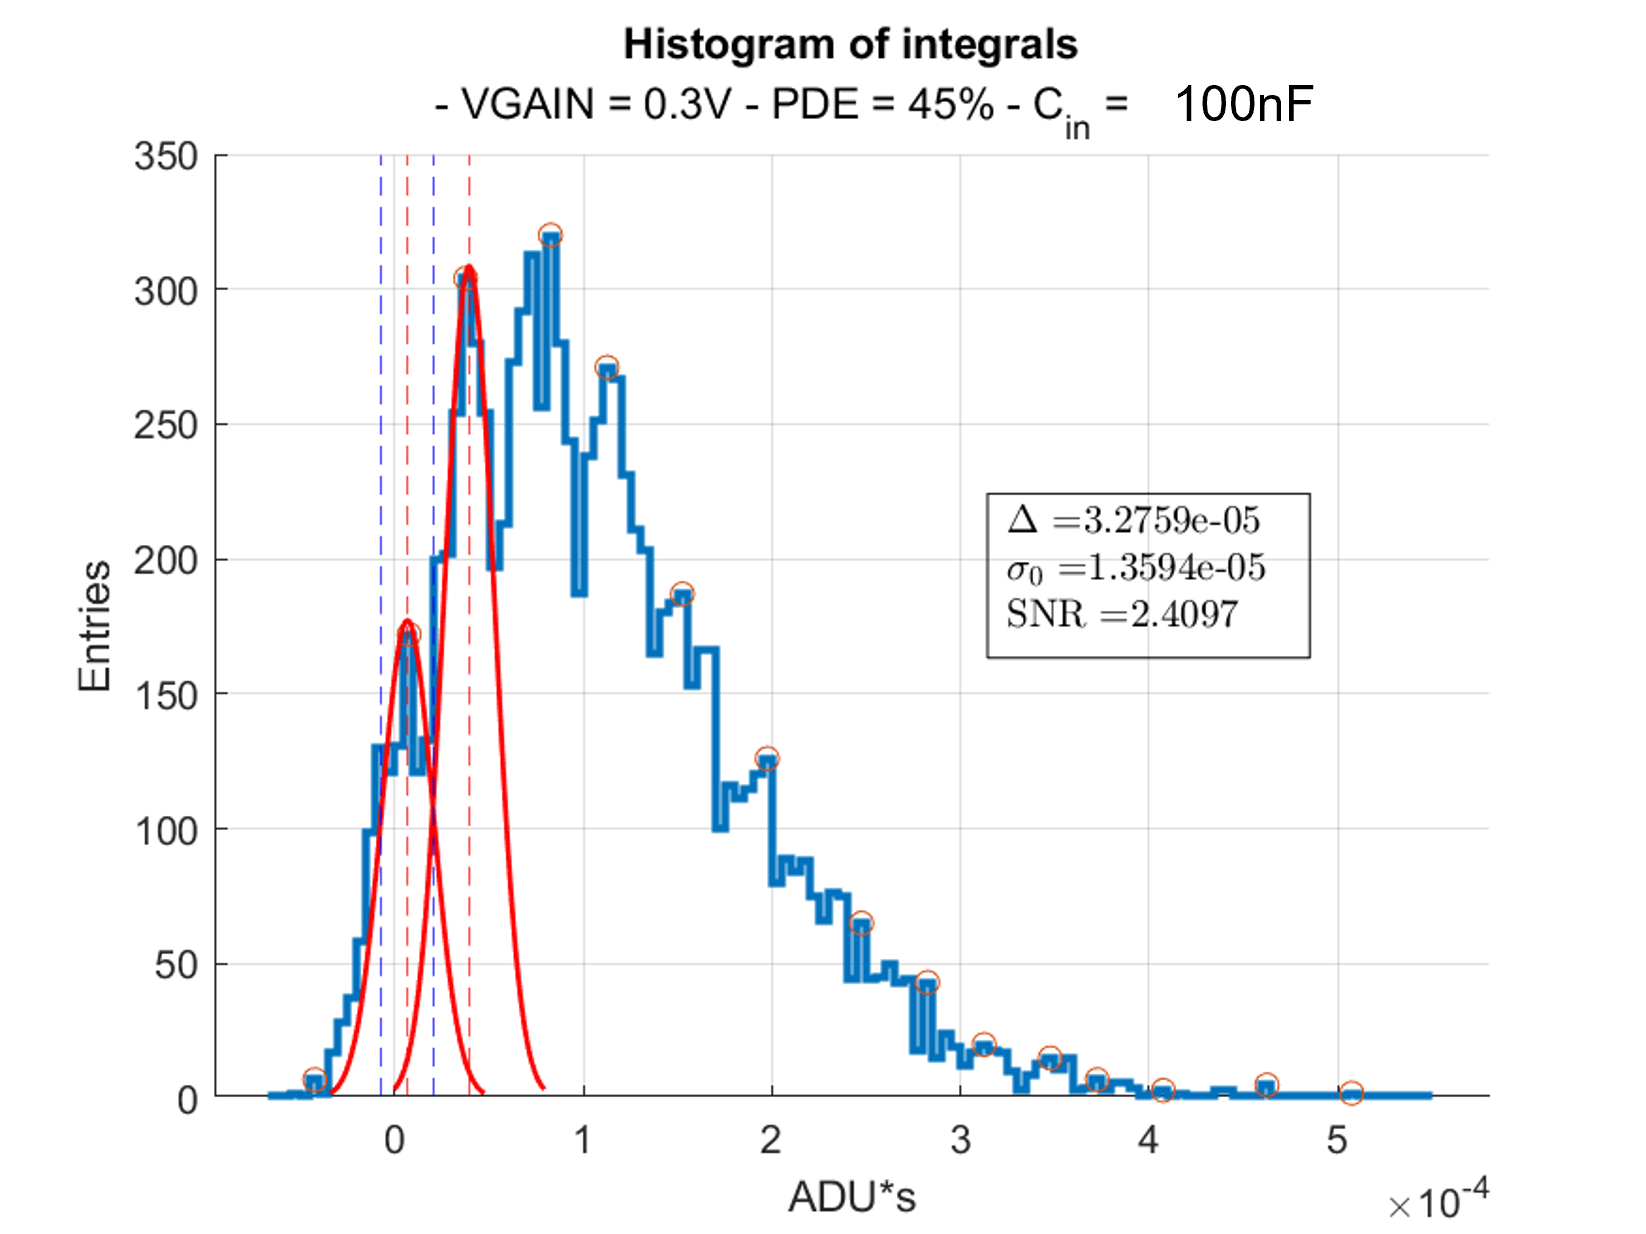
\includegraphics[width=60mm]{Images/hist_noise_int_off.png}}
\caption[]{Effect of turning OFF the AFE integrators.  a) Input frequency spectrum. b) Histogram of charge integrals for a VGAIN = 0.3V configuration.}
\label{fig:fbk_noise_1f}
\end{figure}

The proposed solution to this issue was to develop IIR digital filters inside the FPGA that emulate the response of the AFE integrators with the capability to recover the pedestal value. Figure \ref{fig:dig} shows the block design of the implemented filter inside DAPHNE's FPGA. This filter has two main modules, a low pass filter LPF and a high pass filter HPF. Data from AFE5808's ADC (X[15:0]) enters the LPF, where an average of $2^n$ samples is performed ($n$ is configurable and set to 21). The average value gets substracted from the data and the result is fed to the HPF with filter coefficients to emulate the response of the AFE integrators. Finally, the average value is added back to the filtered data to recover the pedestal. The filter hast two outputs, pedestal recovered and pedestal removed, where the latter is the waveform centered around zero.   

\begin{figure}[h]
\centering
\includegraphics[width=120mm]{Images/digital_filter_1.png}
\caption[]{Digital filter implemented in the FPGA.}
\label{fig:dig}
\end{figure}

Figure \ref{fig:fbk_filtered} shows the response of the implemented filter. Although the filter behaves in the same way as the AFE integrator filters, as can be seen in figure \ref{fig:fbk_filtered}b where a comparison is made between data acquired with the AFE integrators OFF, AFE integrators ON, filtered offline and filtered online in the FPGA; the histogram in figure \ref{fig:fbk_filtered}b shows a deterioration in the SNR of around 0.5.

\begin{figure}[h]
\centering
\subfigure[]{\includegraphics[width=60mm]{Images/hist_fbk_filtered.png}}
\subfigure[]{\includegraphics[width=60mm]{Images/avg_filtered.png}}
\caption[]{FBK-3T SiPMs implemented filter response.  a) Histogram of charge integrals. b) Average single P.E.}
\label{fig:fbk_filtered}
\end{figure}

\subsection{DAPHNE triggering capabilities}

To test DAPHNE triggering capabilities, the cold amplifier was connected to a X-ARAPUCA supercell ganging 48 Hamamatsu SiPMs submerged in $LN_2$. In the same manner as the FBK SIPMs, the Hamamatsu SiPMs were illuminated with the LED driver via an optical fiber, to acquire data with the external trigger and the implemented internal self-trigger. 

First, in order to have raw data, waveforms were acquired using the external trigger with the AFE integrators OFF. The acquired data was also used to confirm that Hamamatsu SiPMs behave similarly to FBK-3T producing SNR and DR values in the same order. Figure \ref{fig:hpk_hist_avg} shows that a $SNR = 4.5$ and a $DR = 2003$ is obtained with a configuration of $PDE = 45\%$ and $VGAIN = 0.89V$. In figure \ref{fig:hpk_filt_comp}, a comparison between the implemented FPGA filter and the AFE integrators is presented at a $PDE = 50\%$. This comparison is made at a $PDE = 50\%$ instead of $45\%$ to have a better resolution, since the peaks are more defined with larger overvoltage values. The result is consistant with FBK measurements, the implemented FPGA filter has a reduced SNR value of around 0.5 compared with the AFE integrator filters and should expect that at $PDE = 45\%$, the SNR value is around 4.   

Until now, waveforms were acquired using the external trigger signal synchronized with the LED driver. In order to have self-trigger capabilities, i.e. that DAPHNE acquires waveforms at a configured P.E. level using as a reference the streaming ADC data, a trigger processor module has to be implemented inside the FPGA that asserts the trigger flag at the correct P.E. level. The fist versions of such module was implemented, simulated and tested. 

\begin{figure}[h]
\centering
\subfigure[]{\includegraphics[width=60mm]{Images/hpk_hist_45.png}}
\subfigure[]{\includegraphics[width=60mm]{Images/hpk_avg_45.png}}
\caption[]{Hamamatsu SiPMs integration test with VGAIN = 0.89V and 45\% PDE.  a) Histogram of charge integrals. b) Average single P.E.}
\label{fig:hpk_hist_avg}
\end{figure}

\begin{figure}[h]
\centering
\subfigure[]{\includegraphics[width=60mm]{Images/hpk_hist_50_filtered.png}}
\subfigure[]{\includegraphics[width=60mm]{Images/hpk_hist_50.png}}
\caption[]{Hamamatsu SiPMs implemented filter response.  a) Histogram of charge integrals - FPGA filtered. b) Histogram of charge integrals - AFE integrators ON.}
\label{fig:hpk_filt_comp}
\end{figure}

Figure \ref{fig:trigger_processor} shows the schematic for the implemented trigger processor. It consist of three main modules: an integrator filter that approximates the behavior of a moving average filter; a threshold detector that assert a signal when the filtered data goes beyond a configured value; and a zero crossing detector module that performs a constant fraction discriminator and asserts a signal when the zero-crossing is detected. 

\begin{figure}[h]
\centering
\includegraphics[width=120mm]{Images/trigger_processor.png}
\caption[]{Scheme of the trigger processor implemented in DAPHNE's FPGA.}
\label{fig:trigger_processor}
\end{figure}

The coincidence of the assertion flags signals a trigger condition that is fed to the external modules that handle the storage of the acquired data. The integrator filter is implemented using the same architecture as the HPF in figure \ref{fig:dig}, using different coefficients. The input of the module is the "pedestal removed" signal from the FPGA digital filter. The integrator filter approximates the response of a moving average filter of 25 samples, just as the integration window shown in figure \ref{fig:filter_figures}a. The peak value of the filtered waveform is equal to the integration process, as can be noted by the red dashed lines. Figure \ref{fig:filter_figures}c shows the histogram of the peak values where the obtained SNR value is around 4.15.

The output of the integrator filter is fed to the threshold detector module and the zero crossing detector module. The threshold detector module is very straightforward, it asserts the threshold flag when the input value is greater than the configured threshold value. The threshold value can be tuned using the histogram shown in figure \ref{fig:filter_figures}c. The mean values of the fitted Gaussian peaks can be considered as the $n$ P.E. value and the intersection of the curves can be considered $n + 1/2$ P.E.  

The zero crossing module deals with the known problem of amplitude walk. If a simple threshold flag is used for triggering, the asserted signal will have a time jitter caused by the fact that the integrated signal has the same rise time always, and is independent of the amplitude, hence small P.E. signals will take longer to reach the threshold value than larger P.E. signals. The module takes the input signal, inverts and delays it; and then performs the subtraction from the original signal, creating a bipolar signal. The zero crossing time of the bipolar signal is time independent of the amplitude. Figure \ref{fig:filter_figures}b show the described process for a delay of 40 samples. Later studies showed that keeping the delay value below the distance between 10\% to 90\% yields the best results minimizing the jitter. The jitter studies are not included in this report but will be presented later on. 


\begin{figure}[h]
\centering
\subfigure[]{\includegraphics[width=60mm]{Images/avg_movmean.png}}
\subfigure[]{\includegraphics[width=60mm]{Images/zero_crossing.png}}
\subfigure[]{\includegraphics[width=60mm]{Images/histogram_movmean_avg.png}}
\subfigure[]{\includegraphics[width=60mm]{Images/hpk_level_11_1_5PE.png}}
\caption[]{Trigger processor integration process. a) Average input waveform and a comparison of the result of the integrator filter and a classic moving average filter. b) Zero crossing detector process. c) Histogram of charge integrals - Peak value of the integrator filter. d) Hardware behavioral simulation - Peak values of the triggered signals.}
\label{fig:filter_figures}
\end{figure}

To test the trigger processor module, a behavioral simulation of the implemented hardware was performed in Iverilog using the raw unfiltered data. The simulation takes the raw unfiltered data and outputs the trigger flag as a boolean vector. In this way, it is know at what point exactly the trigger was asserted compared to the LED reference. Also, it is possible to obtain the intermediate waveforms, such as the output waveform of the integrator module inside the trigger processor and elaborate the histogram shown in blue in figure \ref{fig:filter_figures}d. Then, taking the values that asserted the trigger, the histogram in red is elaborated and is clearly visible that the module triggered at the desired location, calibrated at 11 $ADUs$, corresponding to 1.5 P.E.  

\begin{figure}[h]
\centering
\subfigure[]{\includegraphics[width=60mm]{Images/avg_self_trigger.png}}
\subfigure[]{\includegraphics[width=60mm]{Images/self_trigger_comp.png}}
\caption[]{Self-trigger test with Hamamatsu supercell. a) Average waveform of the first self-triggered integral peak. b) Histograms of charge integrals}
\label{fig:self_trigger_test}
\end{figure}

The test of the self-trigger module with the cold amplifier was performed with the Hamamatsu supercell at $45\%$ PDE. Due to an error loading the incorrect firmware, the trigger was set to 1.8 P.E., calibration of 1.5 P.E. intended for a $50\%$ PDE. Nevertheless, the module behaved as expected. Figure \ref{fig:self_trigger_test} show the results of the test, were a dynamic range of 995 was obtained using the average signal of the first peak of the histogram shown in red in figure \ref{fig:self_trigger_test}b.

According to the simulations, the cut at 1.8 P.E. in the red histogram should be more pronounced, but obtaining a good precise histogram is difficult due to the jitter introduced by the self-trigger, that according to the simulation is around 10 samples.

\label{sec:testing}

\section{DAPHNE plans}
\label{sec:futureplans}

\appendix

\section{Power Consumption}
\label{sec:Power_Consumption}

Using an FPGA power estimator tool, we have estimated that our FPGA will consume about 3.5 Watts and that our AFEs at about 150mW/channel and at 40 channels will consume about 6 Watts. Our cooling fan is estimated to consume about 1.6W of power as well. We estimate that our board will consume about 26 W total. 

\subsection{Power Distribution: }

To generate the bias voltage, a Cockcroft-Walton (CW) Generator is used. +/-10V is generated from the secondary winding of the main power transformer on DAPHNE. This voltage is then fed to the CW Generator . It is possible to choose what bias voltage will be generated. +34V, +45V, +55V, +66V, and +77V can all be chosen.
\\*
\\* Voltages generated for the FPGA are described below in the Power-on Sequence subsection. Voltages generated for the various op-amps are shown in the power distribution diagram. 

\subsection{Power Connectors: }

The DAPHNE board power distribution has similarities to the Mu2E CRV Front End Board. One of the similarities is that they both have a power barrel connector for bench top testing. 
But DAPHNE also needs a different power connector. There are some options. A bulkhead connector, wires, mounted male connector and female mate could be used similar to the alternative to HDMI connectors described above. 
Another option is to use a molex through hole connector with a center pin of 0.156”. Such connectors have been used on boards for CDMS and Mu2E.

\subsection{Cooling Fan: }

For a cooling fan we have decided to use a brushless axial ball bearing flow 5V fan, EFB0405VHD-F00, by Delta Electronics.  We will use a 3 pin connector to connect to the fan: +5V, GND, and Frequency Generator (FG). The FG produces a square wave signal with a frequency that is proportional to the fan speed. This signal is sent to the microcontroller and can allow for detection of low supply voltage or blocked airflow. The use of this function will be optional, and programming will be needed within the microcontroller. 
This fan also includes a surface mount fuse rated for 500mA, 0154.500DR. For now, the plan is to keep the fan constantly turned on once plugged in. This fan has a life expectancy of about 70,000 hours (7.99 years) under continuous operation at 104° F (40°C). 


\subsection{FPGA Power-on Sequence: }

The recommended power-on sequence to achieve minimum current draw for the GTP transceivers is:
\\*
\\*VCCINT (1V) – Internal Supply Voltage
\\*VCCBRAM (1V) – Supply Voltage for block RAM memories
\\*VMGTAVCC (1V) – Analog Supply for the GTP circuits
\\*VMGTAVTT (1.2V) – Analog Supply for the GTP termination circuits
\\*VCCAUX (1.8V) – Auxiliary Supply Voltage
\\*VCCO (2.5V, 3.3V)– Output Drivers Supply Voltage For I/O Banks
\\*
\\*Both VMGTAVCC and VCCINT can be ramped simultaneously. The recommended
power-off sequence is the reverse of the power-on sequence to achieve minimum current draw. The reason for using a linear regulator for  MGTAVCC is because it is very sensitive to noise.
\\*
\\*In the NEXYS video schematic, which uses the same FPGA, an input of 12V is used. In our case we will be using an input of about 8V (same as from Sten’s Mu2E FEB power scheme). 
\\*
\\*The three devices that power the FPGA are the:
 ADP2325 which supplies 1V(5A) and 2.5V(500mA)
LTC3868 which supplies 1.8V(5A) and 3.3V(3.5A)
TPS7A91 which supplies 1V(1A) and 1.2V(1A). 
The 1V is for VMGTAVCC and the  1.2V is for VMGTAVTT, both required for the GTP transceiver. VMGTAVCC is the Analog supply voltage for the GTP transmitter and receiver circuits. VMGTAVTT is the Analog supply voltage for the GTP transmitter and receiver termination circuits. 
\\*
\\*No external device is used to create this sequence. 
The sequencing is done using the enable pins on the voltage regulators. And all of these voltages except VMGTAVTT and VMGTAVCC have a ramp time of 8ms.


\acknowledgments

This is the most common positions for acknowledgments. A macro is
available to maintain the same layout and spelling of the heading.

\paragraph{Note added.} This is also a good position for notes added
after the paper has been written.

\bibliography{DAPHNE_Bib}

% We suggest to always provide author, title and journal data:
% in short all the informations that clearly identify a doc

\end{document}
